% Template for PLoS
% Version 3.5 March 2018
%
% % % % % % % % % % % % % % % % % % % % % %
%
% -- IMPORTANT NOTE
%
% This template contains comments intended
% to minimize problems and delays during our production
% process. Please follow the template instructions
% whenever possible.
%
% % % % % % % % % % % % % % % % % % % % % % %
%
% Once your paper is accepted for publication,
% PLEASE REMOVE ALL TRACKED CHANGES in this file
% and leave only the final text of your manuscript.
% PLOS recommends the use of latexdiff to track changes during review, as this will help to maintain a clean tex file.
% Visit https://www.ctan.org/pkg/latexdiff?lang=en for info or contact us at latex@plos.org.
%
%
% There are no restrictions on package use within the LaTeX files except that
% no packages listed in the template may be deleted.
%
% Please do not include colors or graphics in the text.
%
% The manuscript LaTeX source should be contained within a single file (do not use \input, \externaldocument, or similar commands).
%
% % % % % % % % % % % % % % % % % % % % % % %
%
% -- FIGURES AND TABLES
%
% Please include tables/figure captions directly after the paragraph where they are first cited in the text.
%
% DO NOT INCLUDE GRAPHICS IN YOUR MANUSCRIPT
% - Figures should be uploaded separately from your manuscript file.
% - Figures generated using LaTeX should be extracted and removed from the PDF before submission.
% - Figures containing multiple panels/subfigures must be combined into one image file before submission.
% For figure citations, please use "Fig" instead of "Figure".
% See http://journals.plos.org/plosone/s/figures for PLOS figure guidelines.
%
% Tables should be cell-based and may not contain:
% - spacing/line breaks within cells to alter layout or alignment
% - do not nest tabular environments (no tabular environments within tabular environments)
% - no graphics or colored text (cell background color/shading OK)
% See http://journals.plos.org/plosone/s/tables for table guidelines.
%
% For tables that exceed the width of the text column, use the adjustwidth environment as illustrated in the example table in text below.
%
% % % % % % % % % % % % % % % % % % % % % % % %
%
% -- EQUATIONS, MATH SYMBOLS, SUBSCRIPTS, AND SUPERSCRIPTS
%
% IMPORTANT
% Below are a few tips to help format your equations and other special characters according to our specifications. For more tips to help reduce the possibility of formatting errors during conversion, please see our LaTeX guidelines at http://journals.plos.org/plosone/s/latex
%
% For inline equations, please be sure to include all portions of an equation in the math environment.  For example, x$^2$ is incorrect; this should be formatted as $x^2$ (or $\mathrm{x}^2$ if the romanized font is desired).
%
% Do not include text that is not math in the math environment. For example, CO2 should be written as CO\textsubscript{2} instead of CO$_2$.
%
% Please add line breaks to long display equations when possible in order to fit size of the column.
%
% For inline equations, please do not include punctuation (commas, etc) within the math environment unless this is part of the equation.
%
% When adding superscript or subscripts outside of brackets/braces, please group using {}.  For example, change "[U(D,E,\gamma)]^2" to "{[U(D,E,\gamma)]}^2".
%
% Do not use \cal for caligraphic font.  Instead, use \mathcal{}
%
% % % % % % % % % % % % % % % % % % % % % % % %
%
% Please contact latex@plos.org with any questions.
%
% % % % % % % % % % % % % % % % % % % % % % % %

\documentclass[10pt,letterpaper]{article}
\usepackage[top=0.85in,left=2.75in,footskip=0.75in]{geometry}

% amsmath and amssymb packages, useful for mathematical formulas and symbols
\usepackage{amsmath,amssymb}

% Use adjustwidth environment to exceed column width (see example table in text)
\usepackage{changepage}

% Use Unicode characters when possible
\usepackage[utf8x]{inputenc}

% textcomp package and marvosym package for additional characters
\usepackage{textcomp,marvosym}

% cite package, to clean up citations in the main text. Do not remove.
\usepackage{cite}

% Use nameref to cite supporting information files (see Supporting Information section for more info)
\usepackage{nameref,hyperref}

% line numbers
\usepackage[right]{lineno}

% ligatures disabled
\usepackage{microtype}
\DisableLigatures[f]{encoding = *, family = * }

% color can be used to apply background shading to table cells only
\usepackage[table]{xcolor}

% array package and thick rules for tables
\usepackage{array}

\usepackage{color,soul}
\usepackage[normalem]{ulem}
\usepackage{algorithm}
\usepackage[noend]{algpseudocode}


\usepackage{mhchem}
\usepackage{mathtools}

\DeclarePairedDelimiter\ceil{\lceil}{\rceil}
\DeclarePairedDelimiter\floor{\lfloor}{\rfloor}


% create "+" rule type for thick vertical lines
\newcolumntype{+}{!{\vrule width 2pt}}

% create \thickcline for thick horizontal lines of variable length
\newlength\savedwidth
\newcommand\thickcline[1]{%
  \noalign{\global\savedwidth\arrayrulewidth\global\arrayrulewidth 2pt}%
  \cline{#1}%
  \noalign{\vskip\arrayrulewidth}%
  \noalign{\global\arrayrulewidth\savedwidth}%
}

% \thickhline command for thick horizontal lines that span the table
\newcommand\thickhline{\noalign{\global\savedwidth\arrayrulewidth\global\arrayrulewidth 2pt}%
\hline
\noalign{\global\arrayrulewidth\savedwidth}}


% Remove comment for double spacing
%\usepackage{setspace}
%\doublespacing

% Text layout
\raggedright
\setlength{\parindent}{0.5cm}
\textwidth 5.25in
\textheight 8.75in

% Bold the 'Figure #' in the caption and separate it from the title/caption with a period
% Captions will be left justified
\usepackage[aboveskip=1pt,labelfont=bf,labelsep=period,justification=raggedright,singlelinecheck=off]{caption}
\renewcommand{\figurename}{Fig}

% Use the PLoS provided BiBTeX style
\bibliographystyle{plos2015}


% Remove brackets from numbering in List of References
\makeatletter
\renewcommand{\@biblabel}[1]{\quad#1.}
\makeatother



% Header and Footer with logo
\usepackage{lastpage,fancyhdr,graphicx}
\usepackage{epstopdf}
%\pagestyle{myheadings}
\pagestyle{fancy}
\fancyhf{}
%\setlength{\headheight}{27.023pt}
%\lhead{\includegraphics[width=2.0in]{PLOS-submission.eps}}
\rfoot{\thepage/\pageref{LastPage}}
\renewcommand{\headrulewidth}{0pt}
\renewcommand{\footrule}{\hrule height 2pt \vspace{2mm}}
\fancyheadoffset[L]{2.25in}
\fancyfootoffset[L]{2.25in}
\lfoot{\today}

\usepackage{makecell}
\usepackage{gensymb}
\usepackage{rotating}
\usepackage{pdflscape}
\usepackage{multirow}


%% Include all macros below
\newcommand{\lorem}{{\bf LOREM}}
\newcommand{\ipsum}{{\bf IPSUM}}
\newcommand{\angstrom}{\mbox{\normalfont\AA}}

\newenvironment{changemargin}[2]{%
\begin{list}{}{%
\setlength{\topsep}{0pt}%
\setlength{\leftmargin}{#1}%
\setlength{\rightmargin}{#2}%
\setlength{\listparindent}{\parindent}%
\setlength\textit{emindent}{\parindent}%
\setlength{\parsep}{\parskip}%
}%
\item[]}{\end{list}}



\renewcommand{\arraystretch}{1.3}

%% END MACROS SECTION


\begin{document}
\vspace*{0.2in}

% Title must be 250 characters or less.
\begin{flushleft}
{\Large
\textbf\newline{Adaptive dating and fast proposals: revisiting the phylogenetic relaxed clock model} % Please use "sentence case" for title and headings (capitalize only the first word in a title (or heading), the first word in a subtitle (or subheading), and any proper nouns).
}
\newline
% Insert author names, affiliations and corresponding author email (do not include titles, positions, or degrees).
\\
Jordan Douglas\textsuperscript{1,2*},
Rong Zhang\textsuperscript{1,2},
Alexei J. Drummond\textsuperscript{1,2,3},
Remco Bouckaert\textsuperscript{1,2}
\\
\bigskip
\textbf{1} Centre for Computational Evolution,  University of Auckland, Auckland, New Zealand\\
\textbf{2} School of Computer Science, University of Auckland, Auckland, New Zealand\\
\textbf{3} School of Biological Sciences, University of Auckland, Auckland, New Zealand
\\
\bigskip


% Use the asterisk to denote corresponding authorship and provide email address in note below.
* jordan.douglas@auckland.ac.nz


\end{flushleft}
% Please keep the abstract below 300 words
\section*{Abstract}




% Please keep the Author Summary between 150 and 200 words
% Use first person. PLOS ONE authors please skip this step.
% Author Summary not valid for PLOS ONE submissions.   
\section*{Author summary}




\linenumbers

% Use "Eq" instead of "Equation" for equation citations.
\section*{Introduction}


The molecular clock hypothesis states that the evolutionary rates of biological sequences are approximately constant through time \cite{zuckerkandl1962molecular}.
This assumption forms the basis of phylogenetics, under which the evolutionary trees and divergence dates of life forms are inferred from biological sequences, such as nucleic and amino acids \cite{douzery2003local, drummond2006relaxed}.
In Bayesian phylogenetics, these trees and their associated parameters are estimated as probabilitiy distributions \cite{kuhner1995estimating, larget1999markov, mau1999bayesian}. 
Statistical inference can be performed by the Markov chain Monte Carlo (MCMC) algorithm \cite{metropolis53, hastings70} using platforms such as BEAST \cite{drummond2012bayesian}, BEAST2 \cite{bouckaert2019beast}, MrBayes \cite{ronquist2012mrbayes}, and RevBayes \cite{hohna2016revbayes}.



The simplest phylogenetic clock model -- the strick clock -- makes the convenient assumption that the evolutionary rate is constant across all lineages \cite{zuckerkandl1965evolutionary, kuhner1995estimating, larget1999markov}.  % Early examples? 
However, molecular substitution rates are known to vary over time, over population sizes, over evolutionary pressures, and over nucleic acid replicative machineries \cite{gillespie1994causes, woolfit2009effective, loh2010optimization}.
Moreover, any given dataset may be clock-like (where the substitution rate has a small variance across lineages) or non clock-like (a large variance). 
In the latter case, a strict clock is probably not suitable. 



This led to the development of relaxed (uncorrelated) clock models, under which each branch in the phylogenetic tree has its own molecular substitution rate  \cite{drummond2006relaxed}.
Branch rates can be drawn from a range of probability distributions including Log-Normal, Exponential, Gamma, and Inverse-Gamma distributions \cite{drummond2006relaxed, lepage2007general, li2012model}.
This class of models is widely used, and has aided insight into many recent biological problems, including the 2016 Zika virus outbreak \cite{faria2017establishment} and the COVID-19 pandemic \cite{giovanetti2020first}.
% is compatible with increasingly prominent multispecies coalescent models \cite{ogilvie2017starbeast2}, 

Finally, although not the focus of this article, the class of correlated clock models assumes some form of auto-correlation between rates over time. 
The correlation itself can invoke a range of stochastic models, including compound Poisson \cite{huelsenbeck2000compound} and CIR processes \cite{lepage2007general}, or it can exist as a series of local relaxed clocks \cite{drummond2010bayesian}. 
However, due to the correlated and discrete nature of such models, the time until MCMC convergence may be cumbersome, particularly for larger datasets \cite{drummond2010bayesian}.  



With the overwhelming availabilty of biological sequence data, the development of efficient Bayesian phylogenetic methods is more important than ever. 
The performance of MCMC is dependent not only on computational runtime but also the efficacy of an
MCMC setup to achieve its convergence.
A critical task therein lies the further advancement of MCMC operators.
Recent developments in this area include the advancement of guided tree proposals \cite{zhang2020using, meyer2019adaptive, hohna2012guided}, coupled MCMC \cite{altekar2004parallel, muller2019coupled},
adaptive multivariate transition kernels \cite{baele2017adaptive},
and other explorative proposal kernels such as the Bactrian and mirror kernels \cite{yang2013searching, thawornwattana2018designing}.
In the case of clock models, informed tree proposals can account for correlations between substitution rates and divergence times \cite{zhang2020improving}. 
The rate parameterisation itself can also affect the ability to ``mix'' during MCMC \cite{drummond2006relaxed, li2012model, zhang2020improving}. 




While a range of advanced operators and other MCMC optimisation methods have arisen over the years, there has yet to be a widescale performance benchmarking of such methods as applied to the relaxed clock model. 
In this article, we systematically evaluate how the relaxed clock model can benefit from i) adaptive operator weighting, ii) different substitution rate parameterisations,  iii) the use of Bactrian proposal kernels \cite{yang2013searching}, iv) tree operators which account for correlations between substitution rates and times, and v) adaptive multivariate operators \cite{baele2017adaptive}.
The discussed methods are implemented in and compared using BEAST2 \cite{bouckaert2019beast}. 

% phylogenetic model -- and the operators used during MCMC -- to achieve convergence. 
%A great body of research of MCMC performance



% With increasing sequence availability, it is desirable to have faster MCMC
% This can be achieved through faster mixing and better performance (beagle)
% Address modern optimisation speedups - bactrian, AVMVN, + 2 others not covered in this paper including GUIDED tree proposals
% Address various attempts made to optimise clock models (Rong's paper, different parameterisations + 1 other not covered)
% While many ideas have come up over the years, a large scale systematic comparison of which methods yield faster mixing (if there is one) has not been applied


% In this article, benchmark a range of approaches including...





% Results and Discussion can be combined.
\section*{Models} \label{sect:models}



\subsection*{Preliminaries}



Let $\mathcal{T}$ be a binary rooted time tree with $N$ taxa. Let $L$ be the number of sites within the multiple sequence alignment $D$, and let $L_\text{eff}$ be the effective number of sites in the alignment (i.e. the number of unique patterns across all sites in the alignment). The posterior density of a phylogenetic model is described by

\begin{eqnarray}
\label{eq:bayesian}
p(\mathcal{T}, \vec{\mathcal{R}}^{\,}, \sigma, \mu_C, \theta|D) \propto  p(D|\mathcal{T}, r(\vec{\mathcal{R}}^{\,}), \mu_C) \; p(\mathcal{T}|\theta) \;  p(\vec{\mathcal{R}}^{\,} | \sigma) \; p(\sigma) \; p(\mu_C) \; p(\theta).
\end{eqnarray}


$\sigma$ represents clock model related parameters, and $p(\mathcal{T}|\theta)$ is the tree prior where $\theta$ describes further unspecified parameters. 
The tree likelihood $p(D|\mathcal{T}, r(\vec{\mathcal{R}}^{\,}), \mu_C)$ is computed using the tree-peeling algorithm \cite{felsenstein1981evolutionary}, where $\mu_C$ is the overall clock rate and
$\vec{\mathcal{R}}^{\,}$ is a vector of abstracted branch rates which is transformed into real rates by function $r(\vec{\mathcal{R}}^{\,})$. 
Branch rates have a mean of 1 under the prior to avoid non-identifiability with node heights and the clock rate $\mu_C$.
Three methods of representing rates as $\vec{\mathcal{R}}^{\,}$ are presented in \textbf{\nameref{sect:rateparams}}.  





Let $t_i$ be the height (time) of node $i$.
Each node $i$ in $\mathcal{T}$, except for the root, is associated with a parental branch length $\tau_i$ (the height difference between $i$ and its parent)  and a parental branch substitution rate $r_i = r(\mathcal{R}_i)$. 
In a relaxed clock model, each of the $2N-2$ elements in $\vec{\mathcal{R}}^{\,}$ are independently distributed under the prior $p(\vec{\mathcal{R}}^{\,} | \sigma)$.



The posterior distribution is sampled by the Metropolis-Hastings-Green MCMC algorithm \cite{metropolis53, hastings70, green1995reversible},
under which the probability of accepting proposed state $x^\prime$ from state $x$ is equal to:

\begin{eqnarray}
\label{eq:MCMC}
\alpha(x^\prime|x) =  \min\left( 1, \frac{p(x^\prime|D)}{p(x|D)} \; \frac{q(x|x^\prime)}{q(x^\prime|x)} \; |J| \right).
\end{eqnarray}

$q(a|b)$ is the transition kernel: the probability of proposing state $b$ from state $a$.
The ratio between the two $\frac{q(x|x^\prime)}{q(x^\prime|x)}$ is also known as the Hastings ratio \cite{hastings70}.
The determinant of the Jacobian matrix $|J|$ solves the dimension-matching problem for proposals which operate on multiple terms across one or more spaces \cite{green1995reversible, geyer2003metropolis}. 
This term is known as the Green ratio. 




\clearpage
\subsection*{Substitution rate parameterisations}
\label{sect:rateparams}

In Bayesian inference, the way parameters are represented in the model can affect the mixing ability of the model and the meaning of the model itself \cite{gelman2004parameterization}. Three methods for parameterising substitution rates are described below.
 Each parameterisation is associated with i) an abstraction of the branch rate vector $\vec{\mathcal{R}}^{\,}$, ii) some function for transforming this parameter into unabstracted branch rates $r(\vec{\mathcal{R}}^{\,})$, and iii) a prior density function of the abstraction $p(\vec{\mathcal{R}}^{\,} | \sigma) $. 
 The three methods are summarised in \textbf{Fig \ref{fig:rateparams}}.


\begin{figure}[!h]
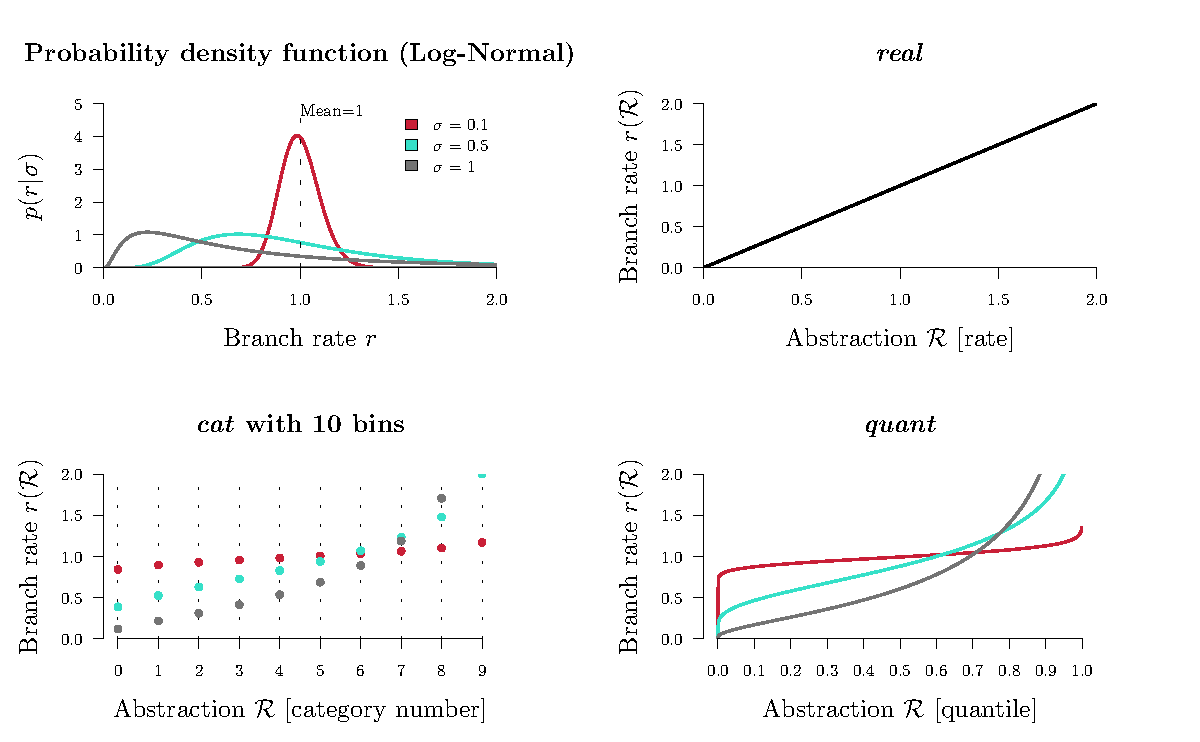
\includegraphics[width=\textwidth]{Figures/rateparameterisation.pdf}
\caption{\textbf{Branch rate parameterisations.} Top left: the prior density of a branch rate $r$ under a Log-Normal($-0.5\sigma^2, \sigma$) distribution (with its mean fixed at 1). 
The function for transforming $\mathcal{R}$ into branch rates $r(\mathcal{R})$ is depicted for \textit{real} (top right), \textit{cat} (bottom left), and \textit{quant} (bottom right).
For simplicity there are 10 \textit{cat} bins displayed, however in practice there are $2N-2$ bins. }
\label{fig:rateparams}
\end{figure}



\clearpage
\subsubsection*{1. Real rates}
The natural (and unabstracted) parameterisation of a substitution rate is a real number $\mathcal{R}_i \in \mathbb{R}, \mathcal{R}_i > 0$ which is equal to the rate itself. Thus, under the \textit{real} parameterisation:

% \vec{\mathcal{R}}^{\,} =& \; \vec{r}^{\,} \\
\begin{align}
r(\vec{\mathcal{R}}^{\,}) =& \; \vec{\mathcal{R}}^{\,}.
\end{align}


Under the Log-Normal clock prior $p(\vec{\mathcal{R}}^{\,} | \sigma)$, rates are distributed with a mean of 1:

\begin{align}
p(\mathcal{R}_i | \sigma) = \frac{1}{\mathcal{R}_i \sigma \sqrt{2\pi}} \exp \big( -\frac{(\ln \mathcal{R}_i - \mu)^2}{2\sigma^2} \big) 
\end{align}


where $\mu = -0.5\sigma^2$ is set such that the expected value of the Log-Normal distribution is 1.
In this article we only consider Log-Normal clock priors, however the methods discussed are general.


Zhang and Drummond 2020 introduced a series of tree operators which propose node heights and branch rates, such that the resulting genetic distances ($r_i \times \tau_i$) remain constant \cite{zhang2020improving}. 
These operators account for correlations between branch rates and branch times.
By keeping the genetic distance of each branch constant, the likelihood is unaltered by the proposal. 


%the correlation between rates and times, as imposed by likelihood function, is r after the proposal , and thus lowers the risk of ``falling o

% Such operators are incompatible with the \textit{cat} parameterisation.  The \textit{real} parameterisation and its associated operators yield a mixing rate up to an order of magnitude faster than that of \textit{cat}. \\




\subsubsection*{2. Categories}
The category parameterisation (\textit{cat}) is an abstraction of the \textit{real} parameterisation. 
Each of the $2N-2$ branches are assigned an integer from $0$ to $n-1$:

\begin{align}
\vec{\mathcal{R}}^{\,} \in& \{ 0, 1, \dotso, n-1 \}^{2N-2}.
\end{align}


These integers correspond to $n$ rate categories (\textbf{Fig. \ref{fig:rateparams}}).
The domain of $\vec{\mathcal{R}}^{\,}$ is uniformly distributed under the prior:


\begin{align}
p(\mathcal{R}_i | \sigma) = p(\mathcal{R}_i) = \frac{1}{n}.
\end{align}



Let $f(x|\sigma)$ be the probability density function (PDF) and let $F(x|\sigma) = \int\limits_{0}^{x} f(t|\sigma) \; dt$ be the cumulative distribution function (CDF) of the prior distribution used by the underlying \textit{real} clock model (a Log-Normal distribution in this project). 
Then, in the \textit{cat} parameterisation, $f(x|\sigma)$ is discretised into $n$ bins and each element within $\vec{\mathcal{R}}^{\,}$ points to one such bin,
where each bin has uniform prior density.
 The rate of each bin is equal to the median value within the bin 


\begin{align}
r(\mathcal{R}_i) =& \; F^{-1}\big(\frac{\mathcal{R}_i + 0.5}{n}\big),
\end{align}

where $F^{-1}$ is the inverse cumulative distribution function (i-CDF).



The key advantage of the \textit{cat} parameterisation is the removal of a term from the posterior density (Equation \ref{eq:bayesian}), or more accurately the replacement of a non-trivial $p(\vec{\mathcal{R}}^{\,} | \sigma)$ term with that of a uniform prior. 
This may facilitate efficient traversal of the parameter space by MCMC.




This parameterisation has been widely used in BEAST and BEAST2 analyses \cite{drummond2006relaxed}. 
However, the recently developed constant distance operators  -- which are incompatible with the \textit{cat} parameterisation -- can yield an increase in mixing rate under \textit{real} by up to an order of magnitude over that of \textit{cat}, depending on the dataset \cite{zhang2020improving}. 






\subsubsection*{3. Quantiles}


Finally, rates can be parameterised as real numbers $0 < \mathcal{R}_i < 1$ which describe the rate's quantile with respect to some underlying clock model distribution. Under the  \textit{quant} parameterisation, each of the $2N-2$ elements in $\vec{\mathcal{R}}^{\,}$ are uniformly distributed.


\begin{align}
\vec{\mathcal{R}}^{\,} \in & \; \mathbb{R}^{2N-2}, 0 < \mathcal{R}_i < 1  \\
p(\mathcal{R}_i | \sigma) = & \; p(\mathcal{R}_i) = 1
\end{align}


Transforming these quantiles into rates invokes the i-CDF of the underlying \textit{real} clock model distribution:


\begin{align}
r(\mathcal{R}_i) =& \; F^{-1}(\mathcal{R}_i).
\end{align}


However, evaluation of the i-CDF is computationally demanding and this may hinder the performance of the \textit{quant} parameterisation.

While this approach has clear similarities with \textit{cat}, the domain of rates here is continuous (as opposed to being confined to a discrete number of bins).
In this project we extended the family of constant distance operators  \cite{zhang2020improving} so they are compatible with \textit{quant} (\textbf{\nameref{sect:S1Appendix}}). 


When $\sigma$ is proposed under either \textit{quant} or \textit{cat}, all of the rates $r(\vec{\mathcal{R}}^{\,})$ are proposed along with it, thus enabling large changes to the state space with a single proposal.
Whereas, this is not the case for \textit{real}, which led to the development of the \texttt{FastClockScale} operator \cite{zhang2020improving}. 








%A potential disadvantage of the \textit{quant} method would be the computational requirements of continuously evaluating the i-cdf.
%As the number of quantiles grows with the taxon count $N$, this drawback would be at its worst on large trees.
%Hence, rather than evaluating the exact i-cdf $F^{-1}$, an approximation $\hat{F}^{-1}$ will be used instead:


%\begin{align}
%r(\mathcal{R}_i) =& \; \hat{F}^{-1}(\mathcal{R}_i).
%\end{align}


%In this article we have extended \textit{quant} through a linear piecewise approximation of the i-cdf. As the piecewise approximation is linear, evaluating the derivatives $\frac{\partial}{\partial \mathcal{R}_i} \hat{F}^{-1}(\mathcal{R}_i) =  D \hat{F}^{-1}(\mathcal{R}_i)$ and $\frac{\partial}{\partial r_i} \hat{F}(r_i) = D \hat{F}(r_i)$  -- which are required for computing the Hastings ratios -- is trivial. The approximation is comprised of $n$ pieces (where $n$ is fixed) and upper and lower rate boundaries $r_\text{min}$ and $r_\text{max}$. The approximation is displayed in \textbf{Fig \ref{fig:rateparams}} and further detailed in \textbf{\nameref{sect:S1Appendix}}.


%Zhang and Drummond 2020 introduced several tree operators for the \textit{real} parameterisation -- including \texttt{Constant Distance}, \texttt{Simple Distance}, and \texttt{Small Pulley}. In this project, we extended these three operators so that they are compatible with the \textit{quant} parameterisation. These are presented in \textbf{\nameref{sect:S1Appendix}}. 





\clearpage
\subsection*{Adaptive operator weighting}
\label{sect:adaptiveSampling}


The weight of an operator determines the probability of the operator being selected at each step during MCMC.
In BEAST2, operators can have a tunable parameter $s$ which determines the step size of the operator \cite{bouckaert2019beast}. 
Although $s$ is learned throughout the MCMC chain, the operator weights themselves are typically held constant.
Pre-existing BEAST2 clock model operators (i.e. those which generate proposals for either $\vec{\mathcal{R}}^{\,}$ or $\sigma$) are summarised in \textbf{Table \ref{table:kernels}}, and further operators are introduced throughout the paper.





% Section intro
% Give some examples of this operator working better on this dataset but not that one, where both operators apply to the same parameter eg. Constant Distance? Any others?
% Bring up theme that this can be related to signal. Sampling from the prior may give better results when there is poor signal, whereas random-walk based operators may do better in the other case. Any general theoretical examples of this?



\begin{table}[h!]
\centering
\begin{tabular}{|l p{4.2cm} l l|} 
 \hline
 Operator & Description & Parameters & Parameterisations  \\
  \hline
 \texttt{RandomWalk} & Moves a single element by a tunable amount. & $\vec{\mathcal{R}}^{\,}, \sigma$ & \textit{cat}, \textit{real}, \textit{quant} \\
  \hline
\texttt{Scale} & Applies \texttt{RandomWalk} on the log-transformation (suitable for parameters with positive domains). & $\vec{\mathcal{R}}^{\,}, \sigma$ & \textit{real}, \textit{quant}  \\
  \hline
 \texttt{Interval} & Applies \texttt{RandomWalk} on the logit-transformation (suitable for parameters with upper and lower limits). & $\vec{\mathcal{R}}^{\,}$ & \textit{quant}  \\
  \hline
 \texttt{Swap} & Swaps two random elements in the vector \cite{drummond2006relaxed}. & $\vec{\mathcal{R}}^{\,}$  & \textit{cat}, \textit{real}, \textit{quant}  \\
 \hline
\texttt{Uniform} & Resamples one element in the vector from a uniform distribution. & $\vec{\mathcal{R}}^{\,}$  & \textit{cat}, \textit{quant}  \\
 \hline
\texttt{ConstantDistance} & Adjusts an internal node height and recalculates all incident branch rates such that the genetic distances remain constant \cite{zhang2020improving}.  & $\vec{\mathcal{R}}^{\,}, \mathcal{T}$ & \textit{real}, \textit{quant} \\
 \hline
\texttt{SimpleDistance} & Applies \texttt{ConstantDistance} to the root node \cite{zhang2020improving}.  & $\vec{\mathcal{R}}^{\,}, \mathcal{T}$ & \textit{real}, \textit{quant} \\
 \hline
\texttt{SmallPulley} & Proposes new branch rates incident to the root such that their combined genetic distance is constant  \cite{zhang2020improving}.  & $\vec{\mathcal{R}}^{\,}$ & \textit{real}, \textit{quant} \\
 \hline
\texttt{FastClockScale} & Applies \texttt{Scale} to $\sigma$ and then recomputes all rates $\vec{\mathcal{R}}^{\,}$ such that their quantiles under the prior $p(\vec{\mathcal{R}}^{\,}|\sigma)$ are constant \cite{zhang2020improving}.  & $\vec{\mathcal{R}}^{\,}, \sigma$ & \textit{real} \\
 \hline
\end{tabular}
\caption{Summary of pre-existing BEAST2 operators, which apply to either branch rates $\vec{\mathcal{R}}^{\,}$ or the clock standard deviation $\sigma$, and the substitution rate parameterisation they apply to.
 \texttt{ConstantDistance} and \texttt{SimpleDistance} also adjust node heights in the tree $\mathcal{T}$. }
\label{table:kernels}
\end{table}







It is not always clear which mixture of operators is best for a given dataset.
In this article we introduce \texttt{AdaptiveOperatorSampler} -- a meta-operator which learns operator weights during MCMC and samples operators according to these weights.
The meta-operator undergoes three phases.
In the first phase (burn-in), \texttt{AdaptiveOperatorSampler} samples from its set of sub-operators uniformly at random.
In the second phase (learn-in), the meta-operator continues to sample operators uniformly at random however it begins learning several terms detailed below.
In its final phase, \texttt{AdaptiveOperatorSampler} samples operators (denoted by $\omega$) using the following distribution:


\begin{align}
\label{eqn:adaptiveSampler}
	p(\omega_i) \propto \begin{cases} 1 & \text{ with probability } \Omega \\ \frac{1}{\mathbb{T}(\omega_i)} \sum\limits_{p \in \text{parameters}} \frac{1}{\sigma^2_p}  \sum\limits_{x \in \text{accepts}_i}  || x_p - x_p^\prime ||^2 & \text{ with probability } 1-\Omega \end{cases}
\end{align}

where $\Omega = 0.01$ allows any sub-operator to be sampled regardless of its performance.
The remaining terms are trained during the second and third phases: the cumulative computational runtime spent on each operator $\mathbb{T}(\omega_i)$, the sample variance $\sigma^2_p$ of each parameter $p$, and the sum-of-squares $\sum\limits_{x \in \text{accepts}_i} ||x_p - x_p^\prime||^2$, where $x_p$ and $x_p^\prime$ are the values of $p$ before and after each acceptance of a proposal made by $\omega_i$. 

%The terms which are learned during the second and third phases are: , 



Under \textbf{Equation \ref{eqn:adaptiveSampler}}, operators which effect larger changes on the parameters of interest, in shorter runtime, are sampled with greater probabilities. 
Division of the sum-of-squares term by the parameter variance $\sigma^2_p$ enables comparison between different parameters.


We also introduce the \texttt{SampleFromPrior($\vec{x}^{\,}$)} operator.
This operator resamples $\psi$ randomly selected elements within vector $\vec{x}^{\,}$ from their prior distributions, where $\psi \sim \text{Binomial}(n=|\vec{x}^{\,}|, p=\frac{s}{|\vec{x}^{\,}|})$ for tunable term $s$.




We hypothesise that datasets with strong signal (or large $L$) will mix best when the more precise and meticulous kind of operator is employed, such as those informed by correlations within the posterior distribution e.g. the family of constant distance operators \cite{zhang2020improving} (\textbf{Fig. \ref{fig:rateparams}}).
Whereas, datasets which contain very poor signal (or small $L$) are likely to mix best when there is more weight placed on bold operators such as \texttt{SampleFromPrior}, \texttt{Swap}, or \texttt{Uniform} which sample each branch rate independently of its current estimate.
Ideally, an operator to the likes of \texttt{AdaptiveOperatorSampler} would learn the combination of weights behind these classes of operators best suited for any given dataset.




\begin{figure}[!h]
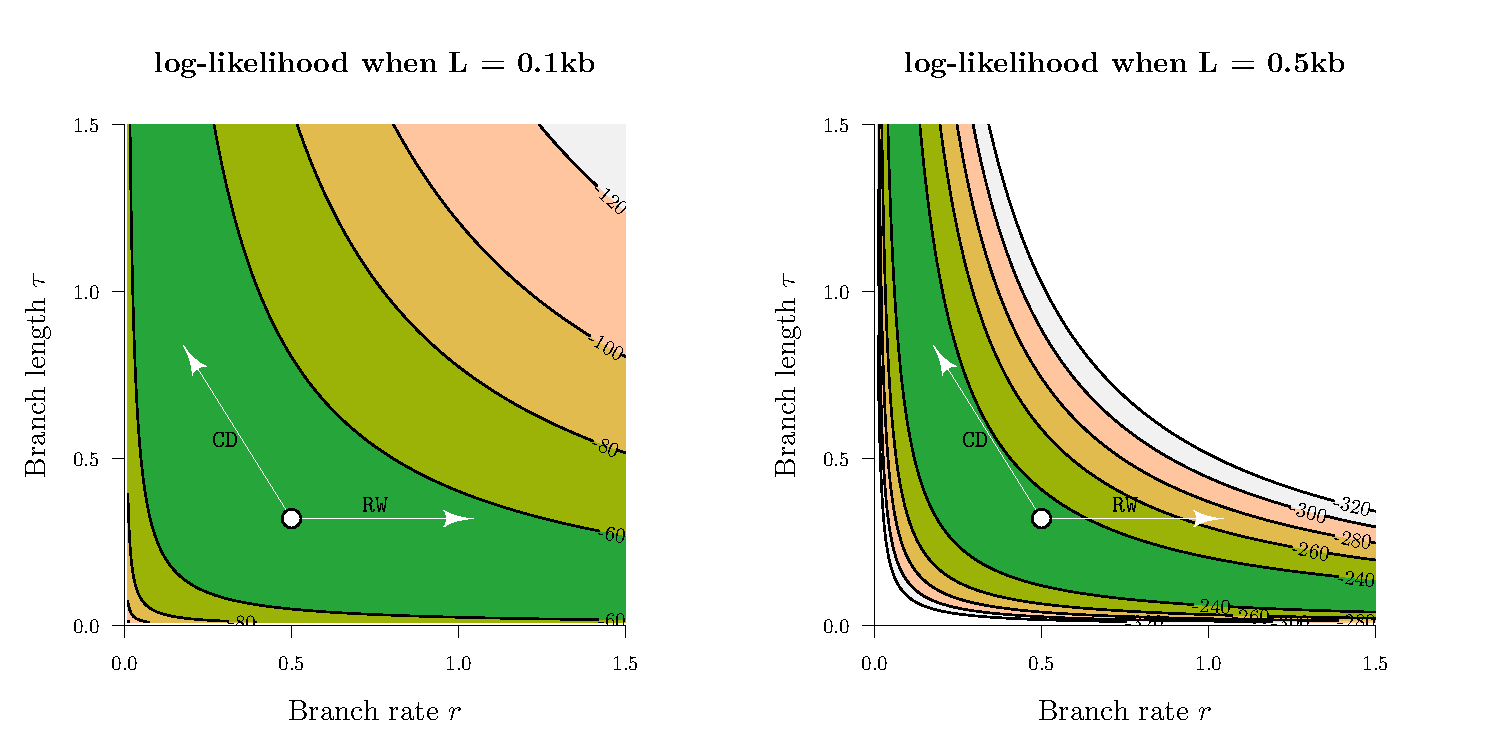
\includegraphics[width=\textwidth]{Figures/correlations.pdf}
\caption{\textbf{Traversing likelihood space.}
The z-axes above are the log-likelihoods of the genetic distance $r \times \tau$ between two simulated nucleic acid sequences of length $L$, under the Jukes-Cantor substitution model \cite{jukes1969evolution}. 
Two possible proposals from the current state (red circle) are depicted.
These proposals are generated by the \texttt{RandomWalk} (\texttt{RW}) and \texttt{ConstantDistance} (\texttt{CD}) operators.
In the low signal dataset ($L=0.1$kb), both operators can traverse the likelihood space effectively.
 However, the exact same proposal by \texttt{RandomWalk} incurs a much larger likelihood penalty in the $L=0.5$kb dataset by ``falling off the ridge'', in contrast to \texttt{ConstantDistance} which ``walks along the ridge''.
 This discrepancy is even stronger for larger datasets and thus necessitates the use of operators such as \texttt{ConstantDistance} which account for correlations between branch lengths and rates. }
\label{fig:rateparams}
\end{figure}


In this article we apply three instances of the \texttt{AdaptiveOperatorSampler} meta-operator to the \textit{real} and \textit{quant} parameterisations. 
These are summarised in \textbf{Table \ref{table:adaptiveSampling}}.



\begin{table}[h!]
\centering
\begin{tabular}{|l p{4cm}|} 
 \hline
 Meta-operator & Operators \\
\hline
 \multirow{4}{*}{\texttt{AdaptiveOperatorSampler($\sigma$)}} & \texttt{FastClockScale($\sigma, \vec{\mathcal{R}}^{\,}$)}$^{*}$ \\ 
 & \texttt{RandomWalk($\sigma$)} \\
 & \texttt{Scale($\sigma$)} \\
 & \texttt{SampleFromPrior($\sigma$)} \\
 \hline
  \multirow{6}{*}{\texttt{AdaptiveOperatorSampler($\vec{\mathcal{R}}^{\,}$)}} & \texttt{ConstantDistance($\vec{\mathcal{R}}^{\,}, \mathcal{T}$)} \\ 
& \texttt{RandomWalk($\vec{\mathcal{R}}^{\,}$)} \\
& \texttt{Scale($\vec{\mathcal{R}}^{\,}$)}$^{*}$ \\
& \texttt{Interval($\vec{\mathcal{R}}^{\,}$)}$^{**}$  \\
& \texttt{Swap($\vec{\mathcal{R}}^{\,}$)} \\
& \texttt{SampleFromPrior($\vec{\mathcal{R}}^{\,}$)} \\
 \hline
   \multirow{2}{*}{\texttt{AdaptiveOperatorSampler(root)}} & \texttt{SimpleDistance($\vec{\mathcal{R}}^{\,}, \mathcal{T}$)} \\ 
&  \texttt{SmallPulley($\vec{\mathcal{R}}^{\,}, t$)}\\
 \hline
\end{tabular}
\caption{Summary of the three instances of \texttt{AdaptiveOperatorSampler} used under the \textit{real} and \textit{quant} parameterisations.
\texttt{AdaptiveOperatorSampler(root)} applies the root-targetting constant distance operators only \cite{zhang2020improving} while \texttt{AdaptiveOperatorSampler($\vec{\mathcal{R}}^{\,}$)} targets all rates and all nodes. 
The two meta-operators are weighted proportionally to the contribution of the root node to the total node count. 
  $^{*}$\textit{real} only. $^{**}$\textit{quant} only. }
\label{table:adaptiveSampling}
\end{table}



%\texttt{AdaptiveOperatorSampler($\sigma$)} samples the clock standard deviation, 
%\texttt{AdaptiveOperatorSampler($\mathcal{R}$)} samples branch rates and internal node heights,
%and \texttt{AdaptiveOperatorSampler(root)} samples  









\clearpage
\subsection*{Bactrian proposal kernel} \label{sect:randomwalks}


%The proposal kernel $q(x^\prime|x)$ defines the conditional probability of proposing state $x^\prime$ given state $x$. 

The step size of a proposal kernal $q(x^\prime|x)$ should be such that the proposed state $x^\prime$ is sufficiently far from the current state $x$ to explore vast areas of parameter space, but not so large that the proposal is rejected too often \cite{roberts1997weak}. 
Operators which attain an acceptance probability of 0.234 are often considered to have arrived at a suitable midpoint between these two extremes \cite{bouckaert2019beast, roberts1997weak}.
The standard uniform distribution kernel has recently been challenged by the Bactrian kernel \cite{yang2013searching, thawornwattana2018designing}.
The $\text{Bactrian}(m)$ distribution is defined as the sum of two Normal distributions:


\begin{align}
	\Sigma \sim \text{Bactrian}(m) \equiv \frac{1}{2}\text{Normal}(-m, 1-m^2) + \frac{1}{2}\text{Normal}(m, 1-m^2)
\end{align}


where $0 \leq m < 1$ describes the modality of the Bactrian distribution. When $m=0$, the Bactrian distribution is equivalent to a $\text{Normal}(0, 1)$ distribution. As $m \rightarrow 1$, the distribution becomes increasingly bimodal (\textbf{Fig. \ref{fig:bactrian}}). 
Yang et al. 2013 \cite{yang2013searching} suggest that $\text{Bactrian}(m=0.95)$ yields a proposal kernel which traverses the posterior distribution more efficiently that the standard uniform kernel, by placing minimal probability on steps which are too small or too large.
In this case, a target acceptance probability of around 0.3 is optimal.


\begin{figure}[!h]
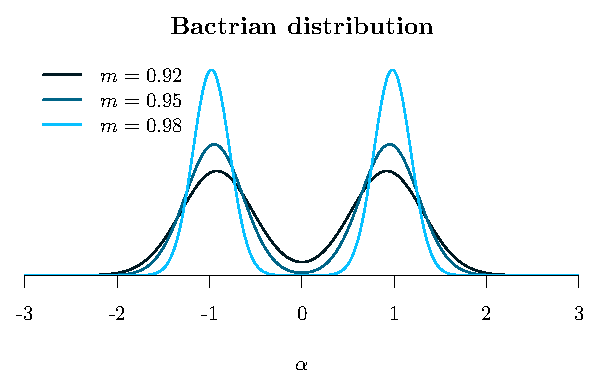
\includegraphics[width=\textwidth]{Figures/bactrian.pdf}
\caption{\textbf{The Bactrian proposal kernel.} The step size made under a Bactrian proposal kernel is equal to $s \Sigma$ where $\Sigma$ is drawn from the above distribution and $s$ is tunable.   }
\label{fig:bactrian}
\end{figure}





In this article we compare the performance of uniform and Bactrian(0.95) proposal kernels with respect to estimating clock model parameters $\vec{\mathcal{R}}^{\,}$ and $\sigma$. 
The clock model operators which these proposal kernels apply to are described in \textbf{Table \ref{table:bactriankernels}}.





\begin{table}[h!]
\centering
\begin{tabular}{|l| p{3cm} l l|} 
 \hline
 & Operator(s) & Proposal & Parameter $x$   \\
  \hline
 1 & \texttt{RandomWalk}  & $x^\prime \leftarrow x + s\Sigma$ & $\vec{\mathcal{R}}^{\,}, \sigma$  \\
  \hline
 2 & \texttt{Scale} & $x^\prime \leftarrow x \times e^{s\Sigma}$ & $\vec{\mathcal{R}}^{\,}, \sigma$   \\
  \hline
 3 & \texttt{Interval} & $\begin{array} {rl} &y \leftarrow \frac{1 - x}{x} \times e^{s\Sigma} \\ &x^\prime \leftarrow \frac{y}{y + 1}  \end{array}$ & $\vec{\mathcal{R}}^{\,}$  \\
  \hline
 4 & \texttt{ConstantDistance} \texttt{SimpleDistance} & $x^\prime \leftarrow x + s\Sigma$ & $t$ \\
 \hline
 5 & \texttt{SmallPulley} & $x^\prime \leftarrow x + s\Sigma$ & $\vec{\mathcal{R}}^{\,}$  \\
 \hline
6 & \texttt{FastClockScale}  & $x^\prime \leftarrow x \times e^{s\Sigma}$ & $\sigma$   \\
 \hline
\end{tabular}
\caption{Proposal kernels $q(x^\prime|x)$ of clock model operators.
 In each operator, $\Sigma$ is drawn from either a $\text{Bactrian}(m)$ or $\text{Uniform}$ distribution. 
 The scale size $s$ is tunable.
 \texttt{ConstantDistance} and \texttt{SimpleDistance} propose tree heights $t$.
  The \texttt{Interval} operator applies to rate quantiles and respects its domain i.e. $0 < x, x^\prime < 1$. }
\label{table:bactriankernels}
\end{table}





% Give the equation of the Uniform + Bactrian kernals
% Fig: Bactrian m=0, 0.92, 0.95, 0.98, + Uniform(-1,1)
% In this article we compare the Uniform + Bactrian proposals in the clock model  

% BRIEFLY describe three operators: random walk, scale, uniform + where the proposal kernal comes in + which parameters in the clock model it applies to



% $x^\prime \leftarrow w \times \frac{u - x}{x - l}$


\clearpage
% REMEMBER to define NNI and SPR acronyms in introduction preferably
\subsection*{Narrow Exchange Rate} \label{sect:NER}

The \texttt{NarrowExchange} operator \cite{drummond2002estimating}, used widely in BEAST \cite{drummond2012bayesian,suchard2018bayesian} and BEAST2 \cite{bouckaert2019beast}, is similar to nearest-neighbour-interchange \cite{semple2003phylogenetics}, and works as follows (\textbf{Fig. \ref{fig:narrowexchange}}):

\textul{\textit{Step 1}}. Sample an internal/root node $E$ from tree $\mathcal{T}$, where $E$ has grandchildren.

\textul{\textit{Step 2}}. Identify the child of $E$ with the greater height. Denote this child as $D$ and its sibling as $C$ (i.e. $t_D > t_C$).

\textul{\textit{Step 3}}. Randomly identify the two children of $D$ as $A$ and $B$.

\textul{\textit{Step 4}}. Relocate the $B-D$ branch onto the $C-E$ branch, so that $B$ and $C$ become siblings and their parent is $D$. All node heights are unchanged.


\begin{figure}[!h]
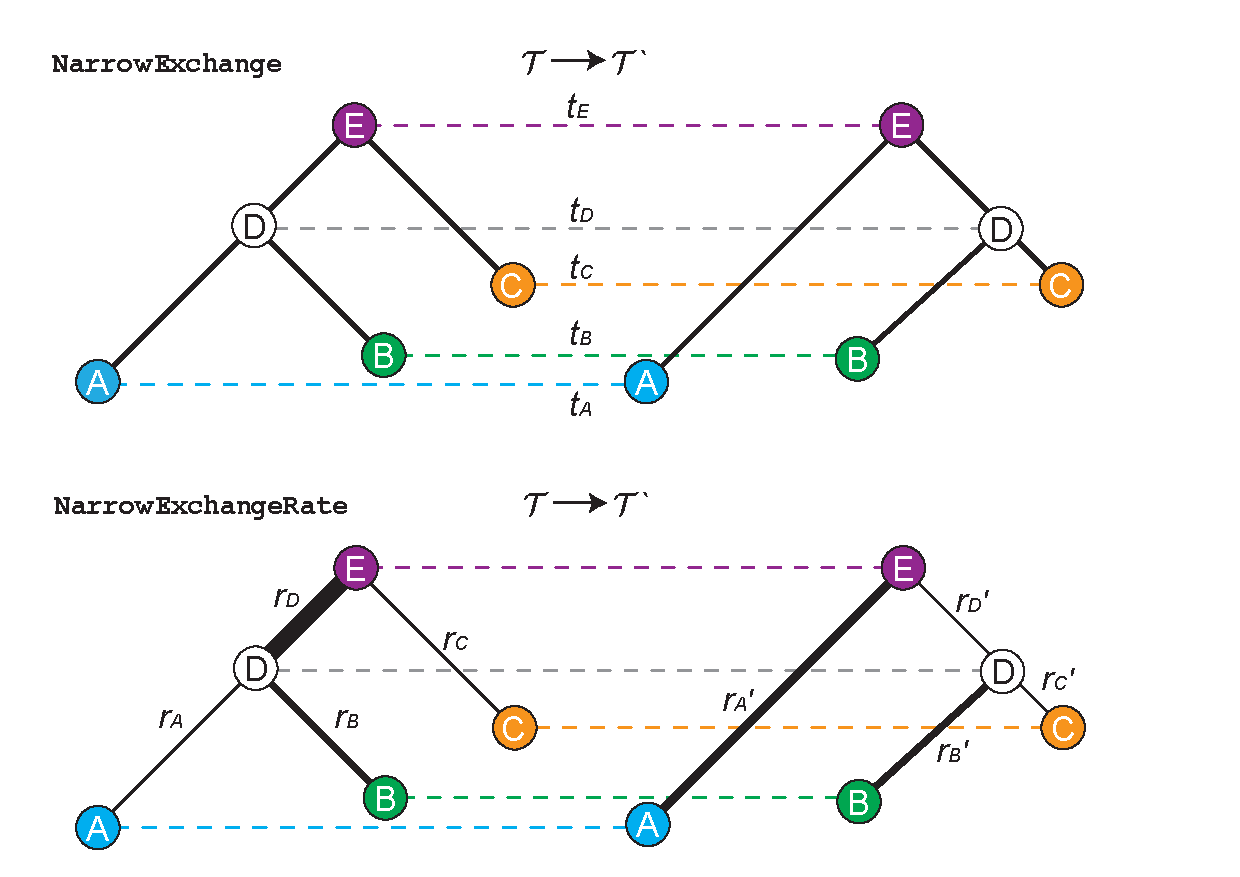
\includegraphics[width=\textwidth]{Figures/NarrowExchange.pdf}
\caption{\textbf{Depiction of \texttt{NarrowExchange} and \texttt{NarrowExchangeRate} operators.} Proposals are denoted by $\mathcal{T} \rightarrow \mathcal{T}^\prime$. The vertical axis corresponds to node height $t$. In the bottom figure, branch rates $r$ are indicated by line thickness. In this example, the $\mathcal{D}_{AE}$ and $\mathcal{D}_{CE}$ constraints are satisfied.}
\label{fig:narrowexchange}
\end{figure}


Lakner et al. 2008 \cite{lakner2008efficiency} found that tree operators which perterb topology (such as nearest-neighbour-interchange and subtree-prune-and-regraft \cite{semple2003phylogenetics}) consistently perform better than those which also change branch lengths (such as LOCAL \cite{simon1998local} and Continuous Change \cite{jow2002bayesian}). 
If \texttt{NarrowExchange} was adapted the relaxed clock model by ensuring that genetic distances remain constant after the proposal (akin to the constant distance operators \cite{zhang2020improving}), then its ability to traverse the state space may improve. 
This may in turn permit proposing a new node height $t_D$ and therefore changing branch lengths.

%Therefore, it seems reasonable to adapt the Narrow Exchange operator for use with the relaxed clock model, such that genetic distances remain constant after performing the proposal $\mathcal{T} \rightarrow \mathcal{T}^\prime$.


Here, we present the \texttt{NarrowExchangeRate} (NER) operator. 
Let $r_A$, $r_B$, $r_C$, and $r_D$ be the clock rates of nodes $A$, $B$, $C$, and $D$, respectively. 
In addition to the modest topological change applied by \texttt{NarrowExchange}, NER also proposes new clock rates ${r_A}^\prime$, ${r_B}^\prime$, ${r_C}^\prime$, and ${r_D}^\prime$. While NER does not alter $t_D$ (i.e. ${t_D}^\prime \leftarrow t_D$), we also consider NERw - a special case of the NER operator which embarks $t_D$ on a random walk:

\begin{align}
	{t_D}^\prime \leftarrow t_D + s\Sigma
\end{align}

for random walk step size $s\Sigma$ where $s$ is a tunable scaler parameter and $\Sigma$ is drawn from a uniform or \textbf{\nameref{sect:randomwalks}}. NER (and NERw) are compatible with both the \textit{real} and \textit{quant} parameterisations. 
Analagous to the \texttt{ConstantDistance} operator, the proposed rates ensure that the genetic distances between nodes $A$, $B$, $C$, and $E$ are constant. 
There are six pairwise distance between these four nodes and therefore six constraints:


\begin{align}
	\mathcal{D}_{AB}: \quad & r_A  (t_D - t_A) + r_B  (t_D - t_B) = \nonumber \\
					 & {r_A}^\prime  (t_E - t_A) + {r_D}^\prime  (t_E - {t_D}^\prime) + {r_B}^\prime ({t_D}^\prime - t_B) \\
	\mathcal{D}_{AC}: \quad & r_A  (t_D - t_A) + r_D  (t_E - t_D) + r_C  (t_E - t_C) = \nonumber \\
				 	  & {r_A}^\prime  (t_E - t_A) + {r_D}^\prime  (t_E - {t_D}^\prime) + {r_C}^\prime ({t_D}^\prime - t_C) \\
 	\mathcal{D}_{AE}: \quad & r_A  (t_D - t_A) + r_D  (t_E - t_D)= \nonumber \\
					  & {r_A}^\prime  (t_E - t_A) \\
  	\mathcal{D}_{BC}: \quad & r_B  (t_D - t_B) + r_D  (t_E - t_D) + r_C  (t_E - t_D)= \nonumber \\
					  & {r_B}^\prime ({t_D}^\prime - t_B) + {r_C}^\prime ({t_D}^\prime - t_C) \\
   	\mathcal{D}_{BE}: \quad & r_B  (t_D - t_B) + r_D  (t_E - t_D)= \nonumber \\
					  & {r_B}^\prime ({t_D}^\prime - t_B) + {r_D}^\prime (t_E - {t_D}^\prime) \\
	\mathcal{D}_{CE}: \quad & r_C  (t_E - t_C)= \nonumber \\
					  & {r_C}^\prime ({t_D}^\prime - t_C) + {r_D}^\prime (t_E - {t_D}^\prime) 
\end{align}


Further constraints are imposed by the model itself:


\begin{align}
	r_i > 0 \text{ and } {r_i}^\prime > 0 \text { for } i \in \{A,B,C,D\} \\
	\max\{t_B, t_C \} < {t_D}^\prime < t_E.
\end{align}



Unfortunately, there is no solution to all six $\mathcal{D}_{ij}$ constraints unless non-positive rates or illegal trees are permitted.
 Therefore rather than conserving all six pairwise distances, NER conserves a \textit{subset} of distances. It is not immediately clear which subset should be conserved. 


\subsubsection*{Automated generation of operators and constraint satisfaction}


The total space of NER operators is comprised of all possible subsets of distance constraints (i.e. $\{\},\{\mathcal{D}_{AB}\}, \{\mathcal{D}_{AC}\}, \dotso , \{\mathcal{D}_{AB}, \mathcal{D}_{AC}, \mathcal{D}_{AE}, \mathcal{D}_{BC}, \mathcal{D}_{BE}, \mathcal{D}_{CE} \}$) which are solvable. 
The simplest NER -- the null operator denoted by NER$\{\}$ -- does not satisfy any distance constraints. 
This is equivalent to \texttt{NarrowExchange}. 
To determine which NER variants have the best performance, we developed an automated pipeline for generating and testing these operators.


\paragraph{1. Solution finding.} Using standard analytical linear-system solving libraries in MATLAB \cite{higham2016matlab}, the $2^6=64$ subsets of distance constraints were solved. 54 of the 64 subsets were found to be solvable, and the unsolvables were discarded.


\paragraph{2. Solving Jacobian determinants.} The determinant of the Jacobian matrix $J$ is required for computng the Green ratio of the proposal. $J$ is defined as 


\begin{align}
	J &= \begin{bmatrix} \frac{\partial {r_A}^\prime}{\partial r_A} & \frac{\partial {r_A}^\prime}{\partial r_B} & \frac{\partial {r_A}^\prime}{\partial r_C} & \frac{\partial {r_A}^\prime}{\partial r_D} \\
	\frac{\partial {r_B}^\prime}{\partial r_A} & \frac{\partial {r_B}^\prime}{\partial r_B} & \frac{\partial {r_B}^\prime}{\partial r_C} & \frac{\partial {r_B}^\prime}{\partial r_D} \\
	\frac{\partial {r_C}^\prime}{\partial r_A} & \frac{\partial {r_C}^\prime}{\partial r_B} & \frac{\partial {r_C}^\prime}{\partial r_C} & \frac{\partial {r_C}^\prime}{\partial r_D} \\
	\frac{\partial {r_D}^\prime}{\partial r_A} & \frac{\partial {r_D}^\prime}{\partial r_B} & \frac{\partial {r_D}^\prime}{\partial r_C} & \frac{\partial {r_D}^\prime}{\partial r_D} \end{bmatrix}.  \nonumber  \\
\end{align}


Computing the determinant $|J|$ invokes standard analytical differentiation and linear algebra libraries of MATLAB. 
6 of the 54 solvable operators were found to have $|J|=0$, corresponding to irreversible proposals, and were discarded. 


\paragraph{3. Automated generation of BEAST2 operators.} Java class files are generated using string processing. Each class corresponds to a single operator, extends the class of a meta-NER-operator, and is comprised of the solutions found in \textbf{1} and the Jacobian determinant found in \textbf{2}. $|J|$ is further augmented if the \textit{quant} parameterisation is employed (\textbf{\nameref{sect:S1Appendix}}).
Two such operators are expressed in \textbf{Algorithms \ref{alg:NER1} and \ref{alg:NER2}}.



\begin{algorithm}
\caption{The NER$\{ \mathcal{D}_{BC}, \mathcal{D}_{CE} \}$ operator.}
\begin{algorithmic}[1]

\Procedure{proposal}{$t_A$, $t_B$, $t_C$, $t_D$, $t_E$, $r_A$, $r_B$, $r_C$, $r_D$}     

	\State
    \State $s\Sigma \leftarrow $ getRandomWalkSize() \Comment{Random walk size is 0 unless this is NERw}
    \State $t_D^\prime \leftarrow t_D + s\Sigma$ \Comment{Propose new node height for $D$}
    \State
    \State $r_A^\prime \leftarrow r_A$ \Comment{Propose new rates}
    \State $r_B^\prime \leftarrow \frac{r_B(t_D - t_B) + r_D(t_E - t_D) + r_D(t_E - t_D^\prime)}{t_D^\prime - t_B}$
    \State $r_C^\prime \leftarrow \frac{r_C(t_E - t_C) - r_D(t_E - t_D^\prime)}{t_D^\prime - t_C}$
    \State $r_D^\prime \leftarrow r_D$
    \State
    \State $|J| \leftarrow \frac{(t_D - t_B)(t_E - t_C)}{(t_D^\prime - t_B)(t_D^\prime - t_C)}$ \Comment{Calculate Jacobian determinant}
    \State \Return $(r_A^\prime, r_B^\prime, r_C^\prime, r_D^\prime, t_D^\prime, |J|)$
    
\EndProcedure

\end{algorithmic}
\label{alg:NER1}
\end{algorithm}


\begin{algorithm}
\caption{The NER$\{ \mathcal{D}_{AE}, \mathcal{D}_{BE}, \mathcal{D}_{CE} \}$ operator.}
\begin{algorithmic}[1]

\Procedure{proposal}{$t_A$, $t_B$, $t_C$, $t_D$, $t_E$, $r_A$, $r_B$, $r_C$, $r_D$}     

	\State
    \State $s\Sigma \leftarrow $ getRandomWalkSize() \Comment{Random walk size is 0 unless this is NERw}
    \State $t_D^\prime \leftarrow t_D + s\Sigma$ \Comment{Propose new node height for $D$}
    \State
    \State $r_A^\prime \leftarrow \frac{r_A(t_D - t_A) + r_D(t_E - t_D)}{t_E - t_A}$ \Comment{Propose new rates}
    \State $r_B^\prime \leftarrow \frac{r_B(t_D - t_B) + r_D(t_D^\prime - t_D)}{t_D^\prime - t_B}$
    \State $r_C^\prime \leftarrow \frac{r_C(t_E - t_C) - r_D(t_E - t_D^\prime)}{t_D^\prime - t_C}$
    \State $r_D^\prime \leftarrow r_D$
    \State
    \State $|J| \leftarrow \frac{(t_D - t_A)(t_D - t_B)(t_E - t_C)}{(t_E - t_A)(t_D^\prime - t_B)(t_D^\prime - t_C)}$ \Comment{Calculate Jacobian determinant}
    \State \Return $(r_A^\prime, r_B^\prime, r_C^\prime, r_D^\prime, t_D^\prime, |J|)$
    
\EndProcedure

\end{algorithmic}
\label{alg:NER2}
\end{algorithm}

The 48 operators generated by this pipeline are evaluated and compared in \textbf{\nameref{sect:results}}. Each operator is considered with and without a random walk on $t_D$ and thus there are 96 total settings.



\clearpage
\subsection*{A guided adaptive leaf rate operator}
\label{AVMVN_sect}

A \textit{guided} operator incorporates knowledge about neighbouring states, while an \textit{adaptive} operator undergoes a training process to improve its efficiency over time \cite{roberts2007coupling}. In previous work, parsimony scores and conditional clade probabilities of neighbouring trees have been employed by guided tree operators \cite{hohna2012guided,zhang2020using,meyer2019adaptive} and the latter has also been explored as the basis of  adaptive tree operators \cite{hohna2012guided,meyer2019adaptive}. The (adaptive) mirror kernel \cite{thawornwattana2018designing} learns a target distribution which acts as a `mirror image' of the current point $x$.  The adaptable variance multivariate normal (AVMVN) kernel \cite{baele2017adaptive,suchard2018bayesian} learns correlations between parameters during MCMC. Baele et al. 2017  observed a large increase ($\approx 5-10 \times$) in sampling efficiency from using the AVMVN kernel on clock rates and substitution model parameters across partitions \cite{baele2017adaptive}.  


In this article we consider application of the AVMVN kernel to the branch rates of leaf nodes. 
This operator, referred to as \texttt{LeafAVMVN}, is not readily applicable to internal node branch rates due to their dependencies on tree topology.  




\subsubsection*{AVMVN kernel}


The AVMVN kernel assumes its parameters live in $x \in \mathbb{R}^N$ and that these parameters follow a Multivariate Normal distribution with covariance matrix $\Sigma_N$. Hence, the kernel operates on the logarithmic or logistic transformation of the $N$ leaf branch rates, depending on the rate parameterisation:

\begin{align}
	x_i = \begin{cases} \log r_i \text{ for } \textit{real} \\
						\log \frac{q_i}{1 - q_i} \text{ for } \textit{quant}  \end{cases}
\end{align}

where $r_i$ is a real rate and $q_i$ is a rate quantile. The AVMVN probability density is defined by 


\begin{align}
	\mathcal{AVMVN}(x) =  \mathcal{MVN}\big(x, (1-\beta) \frac{\Sigma_N}{N} + \beta \frac{\mathbb{I}_N}{N} \big) ,
\end{align}


where $\mathcal{MVN}$ is the Multivariate Normal probability density. $\beta \; (= 0.05)$ is a constant which determines the fraction of the proposal determined by the identity matrix $\mathbb{I}_N$, as opposed to the covariance matrix $\Sigma_D$ which is trained during MCMC.

The AVMVN proposal kernel is computed as


\begin{align}
	x^\prime &\leftarrow x + \sum\limits_{i=1}^N \sum\limits_{j=i}^N c_{i,j} \times s\Sigma \\
	\text {where }  c &= \text{cholesky} \left( (1-\beta) \frac{\Sigma_N}{N} + \beta \frac{\mathbb{I}_N}{N} \right).
\end{align}


The cholesky$(Y)$ decomposition returns a lower diagonal matrix $L$, with positive real diagonal entries, such that $Y = LL^\prime$ \cite{lindstrom1988newton, pourahmadi2007cholesky}. $s$ is a tunable step size parameter and $\Sigma$ is a random variable drawn from a proposal kernel (uniform or Bactrian for instance). Our BEAST2 implementation of the AVMVN kernel is adapted from that of BEAST \cite{suchard2018bayesian}.



In \nameref{sect:results}, we evaluate the \texttt{LeafAVMVN} operator for its ability to estimate leaf rates. 
As the size of the covariance matrix $\Sigma_N$ grows with the number of taxa $N$, AVMVN is hypothesised to work well on small trees but become less efficient with larger taxon sets.







\clearpage
\subsection*{Model specification and MCMC settings} \label{sect:methods}

In all phylogenetic analyses presented here, we use a Yule \cite{yule1925ii} tree prior $p(\mathcal{T}|\lambda)$ with birth rate $\lambda \sim \text{Log-Normal}(1,1.25)$.
The clock standard deviation has a $\sigma \sim \text{Gamma}(0.5396,0.3819)$ prior.
Datasets are partitioned into subsequences, where each partition is associated with a distinct HKY substitution model \cite{hasegawa1985dating}.
The transition-transversion ratio $\kappa \sim \text{Log-Normal}(1, 1.25)$, the four nucleotide frequencies $(f_A, f_C, f_G, f_T) \sim \text{Dirichlet}(10,10,10,10)$, and the relative clock rate $\mu_C \sim \text{Log-Normal}(1, 0.6)$ are estimated independently for each partition.
The operator scheme ensures that the clock rates $\mu_C$ have a mean of 1 across all partitions. 
To enable the rapid benchmarking of larger datasets we use BEAGLE for high-performance tree likelihood calculations \cite{ayres2012beagle} and coupled MCMC with four chains for efficient mixing \cite{muller2019coupled}.
The neighbour joining tree \cite{saitou1987neighbor} is used as the initial state in each MCMC chain.



\clearpage
\section*{Results} \label{sect:results}





\subsection*{Assessment criteria and datasets}






% Cite HKY somewhere hasegawa1985dating


To avoid a cross-product explosion, the five targets for clock model improvement are evaluated sequentially in the following order: \textbf{\nameref{sect:adaptiveSampling}} \textbf{\nameref{sect:rateparams}}, \textbf{\nameref{sect:randomwalks}}, \textbf{\nameref{sect:NER}}, and \textbf{\nameref{AVMVN_sect}}.
The four operators introduced in these sections are summarised in \textbf{Table \ref{table:newOperators}}.
The setting which is considered to be the best in each step is then incorporated into the following step. This protocol and its outcomes are summarised in \textbf{Fig. \ref{fig:tournament}}.



\begin{table}[h!]
\centering
\begin{tabular}{|l p{4cm} l|} 
 \hline
 Operator & Description & Parameters  \\
  \hline
 \texttt{AdaptiveOperatorSampler} & Samples sub-operators proportionally to their weights, which are learned (see \nameref{sect:adaptiveSampling}). & $\vec{\mathcal{R}}^{\,}, \sigma, \mathcal{T}$ \\
  \hline
 \texttt{SampleFromPrior} & Resamples a random number of elements from their prior (see \nameref{sect:adaptiveSampling}). & $\vec{\mathcal{R}}^{\,}, \sigma$ \\
  \hline
 \texttt{NarrowExchangeRate} & Moves a branch and recomputes branch rates so that genetic distances are constant (see \nameref{sect:NER}). & $\vec{\mathcal{R}}^{\,}, \mathcal{T}$\\
  \hline
 \texttt{LeafAVMVN}  & Proposals new rates for all leaves in one move (see \nameref{AVMVN_sect}) \cite{baele2017adaptive}. & $\vec{\mathcal{R}}^{\,}$ \\
  \hline
\end{tabular}
\caption{Summary of clock model operators introduced throughout this article. Pre-existing clock model operators are summarised in \textbf{Table \ref{table:kernels}}}
\label{table:newOperators}
\end{table}



\begin{figure}[!h]
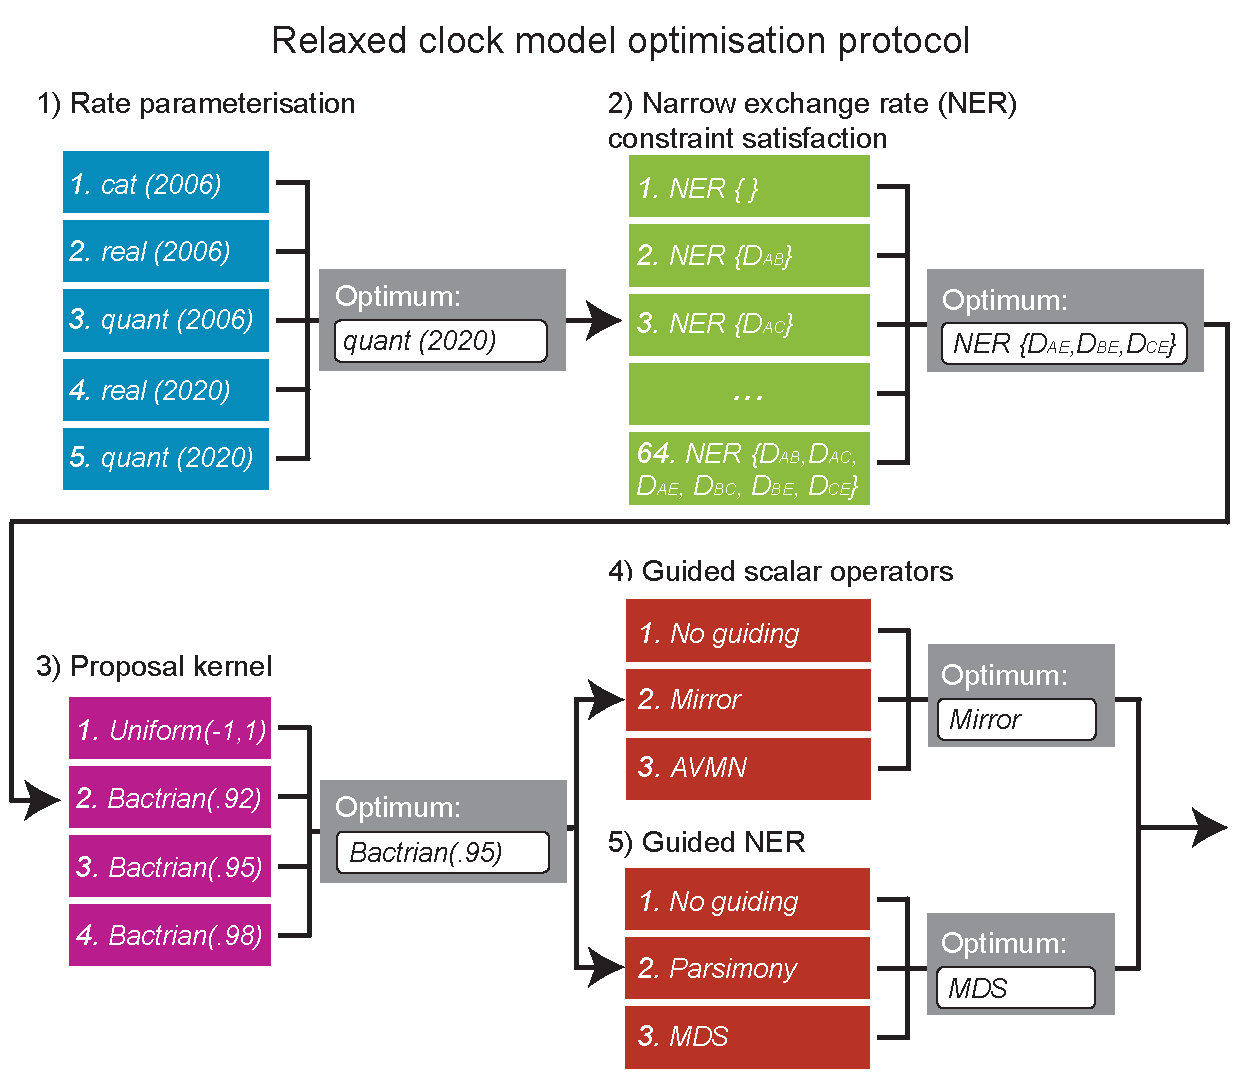
\includegraphics[width=\textwidth]{Figures/tournament.pdf}
\caption{\textbf{Protocol for optimising clock model methodologies.} Each area (detailed in \textbf{\nameref{sect:models}}) is optimised sequentially, and the best setting from each step is used when optimising the following step.}
\label{fig:tournament}
\end{figure}


Methodologies are assessed according to the following criteria.


\textbf{1. Validation}. This is assessed by measuring the coverage of all estimated parameters in a well-calibrated simulation study, using 100 simulated datasets (with $N=100$ taxa and $L=5000$ nucleotide alignments). These are presented in \textbf{\nameref{sect:WCSS_appendix}}. \\


\textbf{2. Mixing of parameters}. Key parameters are evaluated for the number of effective samples generated per hour (ESS/hr). This calculation is performed by BEAST2 \cite{bouckaert2019beast}. \\

%\textbf{3. Time to convergence}. Two independent MCMC chains are run and the time is measured until: a) the absolute difference in clade posterior probability between the two chains is less than 0.05 for all clades, b) the Rubin-Gelman statistic $\hat{R}$ \cite{gelman1992inference} of every estimated parameter is less than 1.05, and c) the effective sample size \cite{rambaut2018posterior} of every estimated parameter is greater than 200 in each chain. \\



Methodologies are benchmarked using one simulated and nine empirical datasets.
The latter were compiled \cite{lanfear2019Github} and partitioned \cite{lanfear2016partitionfinder} by Lanfear et al. as `benchmark alignments' (\textbf{Table \ref{table:datasets}}).
Each methodology is benchmarked across 5 replicates on each dataset, using an the Intel Xeon Gold 6138 CPU (2.00 GHz).
All methodologies use identical models and operator configurations, except where a difference is specified.


%All 25 datasets presented in \textbf{Table \ref{table:datasets}} are benchmarked together $1 \times$ each at the end of the protocol. Datasets and BEAST2 .xml templates are provided in the GitHub repository accompanying this article.



% https://github.com/roblanf/BenchmarkAlignments
\begin{table}[h!]
\centering
\begin{tabular}{|l| l l l l l|} 
 \hline
  & $N$ & $P$ & $L$ (kb) & $L_\text{eff}$ (kb) & \textbf{Description} \\
  \hline
 
 
 1  &  38  &  8  &  9.1  &  6.45  &  Seed plants (Ran 2018 \cite{Ran_2018}) \\ 

2  &  44  &  7  &  5.9  &  1.8  &  Squirrel Fishes (Dornburg 2012 \cite{Dornburg_2012}) \\ 

3  &  44  &  3  &  1.9  &  0.8  &  Bark beetles (Cognato 2001 \cite{Cognato_2001}) \\ 

4  &  51  &  6  &  5.4  &  1.8  &  Southern beeches (Sauquet 2011 \cite{Sauquet_2011}) \\ 

5  &  61  &  8  &  6.9  &  4.3  &  Bony fishes (Broughton 2013 \cite{Broughton_2013}) \\ 

6  &  70  &  3  &  2.2  &  0.9  &  Caterpillars (Kawahara 2013 \cite{Kawahara_2013}) \\ 

7  &  78  &  8  &  3.4  &  3.1  &  Animals (Cannon 2016 \cite{Cannon_2016}) \\ 

8  &  80  &  1 &  10.0  &  4.2  &  \textit{Simulated data}  \\ 

9  &  94  &  4  &  2.2  &  1  &  Bees (Rightmyer 2013 \cite{Rightmyer_2013}) \\ 

10  &  106  &  1  &  0.8  &  0.5  &  Songbirds (Moyle 2016 \cite{Moyle_2016}) \\ 





 \hline
\end{tabular}
\caption{Datasets used during benchmarking, sorted in increasing order of taxa count $N$. Number of partitions $P$, total alignment length $L$, and number of patterns $L_\text{eff}$ are also specified.}
\label{table:datasets}
\end{table}


\clearpage
\subsection*{Round 1: A simple operator-weight learning algorithm can improve performance}

We compared the cons, nocons, and adapt operator configurations for the \textit{real} and \textit{quant} parameterisations (\textbf{Table \ref{table:round1Results}}).
The nocons configuration contained the standard BEAST2 operator mix, while cons contained the operator mix used by Zhang and Drummond 2020 \cite{zhang2020improving}. 
The adapt mix combines the above operators, as well as the rudimentary \texttt{SampleFromPrior} operator, and learns the weights of each operator using  \texttt{AdaptiveOperatorSampler}.


\begin{table}[h!]
\centering
\begin{tabular}{|l l l l|} 
 \hline
Configuration & Operator & Weight & Parameterisations  \\
  \hline
 \multirow{6}{*}{nocons} & \texttt{RandomWalk($\mathcal{R}$)} & $10$ & \textit{real}  \\
 	& \texttt{Scale($\vec{\mathcal{R}}^{\,}$)} & $10$ & \textit{real} \\ 
 	& \texttt{Uniform($\vec{\mathcal{R}}^{\,}$)} & $10$ & \textit{quant} \\ 
 	& \texttt{Interval($\vec{\mathcal{R}}^{\,}$)} & $10$ & \textit{quant} \\ 
 	& \texttt{Swap($\vec{\mathcal{R}}^{\,}$)} & $10$ & \textit{real}, \textit{quant} \\ 
 	& \texttt{Scale($\sigma$)} & $10$ & \textit{real}, \textit{quant} \\ 
  \hline
   \multirow{10}{*}{cons} 
   & \texttt{ConstantDistance($\vec{\mathcal{R}}^{\,}, \mathcal{T}$)} & $20 \times \frac{2N-2}{2N-1}$ & \textit{real}, \textit{quant}  \\
   & \texttt{SimpleDistance($\vec{\mathcal{R}}^{\,}, \mathcal{T}$)} & $10 \times \frac{2N-2}{2N-1}$ & \textit{real}, \textit{quant}  \\
   & \texttt{SmallPulley($\vec{\mathcal{R}}^{\,}$)} & $10 \times \frac{2N-2}{2N-1}$ & \textit{real}, \textit{quant}  \\
   & \texttt{RandomWalk($\vec{\mathcal{R}}^{\,}$)} & $5$ & \textit{real}  \\
 	& \texttt{Scale($\vec{\mathcal{R}}^{\,}$)} & $2.5$ & \textit{real} \\ 
 	& \texttt{Uniform($\vec{\mathcal{R}}^{\,}$)} & $5$ & \textit{quant} \\ 
 	& \texttt{Interval($\vec{\mathcal{R}}^{\,}$)} & $2.5$ & \textit{quant} \\ 
 	& \texttt{Swap($\vec{\mathcal{R}}^{\,}$)} & $2.5$ & \textit{real}, \textit{quant} \\ 
 	& \texttt{FastClockScale($\sigma, \vec{\mathcal{R}}^{\,}$)} & $10$ & \textit{real}  \\ 
 	& \texttt{Scale($\sigma$)} & $10$ &  \textit{quant} \\ 
  \hline
     \multirow{3}{*}{adapt} & \texttt{AdaptiveOperatorSampler($\sigma$)} & $10$ & \textit{real}, \textit{quant} \\
 	& \texttt{AdaptiveOperatorSampler($\vec{\mathcal{R}}^{\,}$)} & $30 \times \frac{2N-2}{2N-1}$ & \textit{real}, \textit{quant} \\
 	& \texttt{AdaptiveOperatorSampler(root)} & $30 \times \frac{1}{2N-1}$ & \textit{real}, \textit{quant} \\
  \hline

\end{tabular}
\caption{Operator configurations for Round 1. In each configuration, the weight behind $\mathcal{R}$ sums to 30 and for $\sigma$ is equal to 10 within any one rate parameterisation. 
Operators which apply to either internal nodes or the root (but not both) are weighted according to leaf count $N$. The adapt operators are further broken down in \textbf{Table \ref{table:adaptiveSampling}}.} 
%The total weight of all operators across all parameters was 116 in each MCMC setup.
T%herefore a weight of 10 corresponds to sampling probability of 0.086, for example.
\label{table:round1Results}
\end{table}




These results show that, while nocons gives better performance than cons on smaller datasets (corresponding to low signal), and cons performs better on larger datasets (high signal), the adapt configuration gives the best performance overall.
This trend is observed for both the \textit{real} and the \textit{quant} parameterisations.
Therefore, the \texttt{AdaptiveOperatorSampler} operator will be included in all subsequent rounds in the tournament. 





\clearpage
\subsection*{Round 2: The \textit{real} parameterisation yields the fastest mixing }

We compared the three rate parameterisations described in \textbf{\nameref{sect:rateparams}}. 
The \textit{cat} operator configuration is described in \textbf{Table \ref{table:round2Results}}.
\textit{real} and \textit{quant} make use of constant distance tree operators \cite{zhang2020improving} and both use the \texttt{AdaptiveOperatorSampler} operator to learn clock model operator weights.
The three settings are validated in \textbf{\nameref{sect:WCSS_appendix}}.




\begin{table}[h!]
\centering
\begin{tabular}{|l l l|} 
 \hline
Configuration & Operator & Weight  \\
  \hline
 \multirow{4}{*}{\textit{cat}} 
 	& \texttt{RandomWalk($\vec{\mathcal{R}}^{\,}$)} & $10$ \\
 	& \texttt{Uniform($\vec{\mathcal{R}}^{\,}$)} & $10$  \\ 
 	& \texttt{Swap($\vec{\mathcal{R}}^{\,}$)} & $10$ \\ 
 	& \texttt{Scale($\sigma$)} & $10$ \\ 
  \hline
\end{tabular}
\caption{Operator configurations for \textit{cat} in Round 2. The configurations of \textit{real} (adapt) and \textit{quant} (adapt) are shown in \textbf{Table \ref{table:round1Results}}.}
\label{table:round2Results}
\end{table}








%\textbf{Fig. \ref{fig:parameterisationResults}} shows that the \textit{real 2006} performs considerably worse than any of the other settings. This is due to the poor sampling of the prior under this setting (i.e. low ESS of $p(\theta)$). The failure of \textit{real 2006} thus highlights the appeal of 1) the \textit{cat} or \textit{quant} parameterisations, both of which have trivial contributions to the prior density (i.e. uniform priors), and 2) the smarter operators used by \textit{real} (Zhang and Drummond 2020). Due to its computational burden, \textit{real 2006} was not benchmarked for all of the datasets in \textbf{Table \ref{table:datasets}}.




%Our results show that the \textit{quant} parameterisation yields the best performance with respect to effective samples per hour. \textit{quant} outperforms \textit{quant 2006}, suggesting that the constant distance operators are effective. Furthermore, \textit{quant} outperforms \textit{real} especially at sampling from the posterior and prior distributions (i.e. high ESS/hr for $p(\theta|D)$ and $p(\theta)$). This is most likely because of the uniform prior distribution of rate quantiles.

%Overall, \textit{quant} yields a median ESS/hr approximately 150 \% faster with respect to sampling the posterior probability, and approximately 30 \% faster with respect to sampling branch rates $r$ and clock standard deviation $\sigma$, compared with \textit{real}.






\begin{figure}[!h]
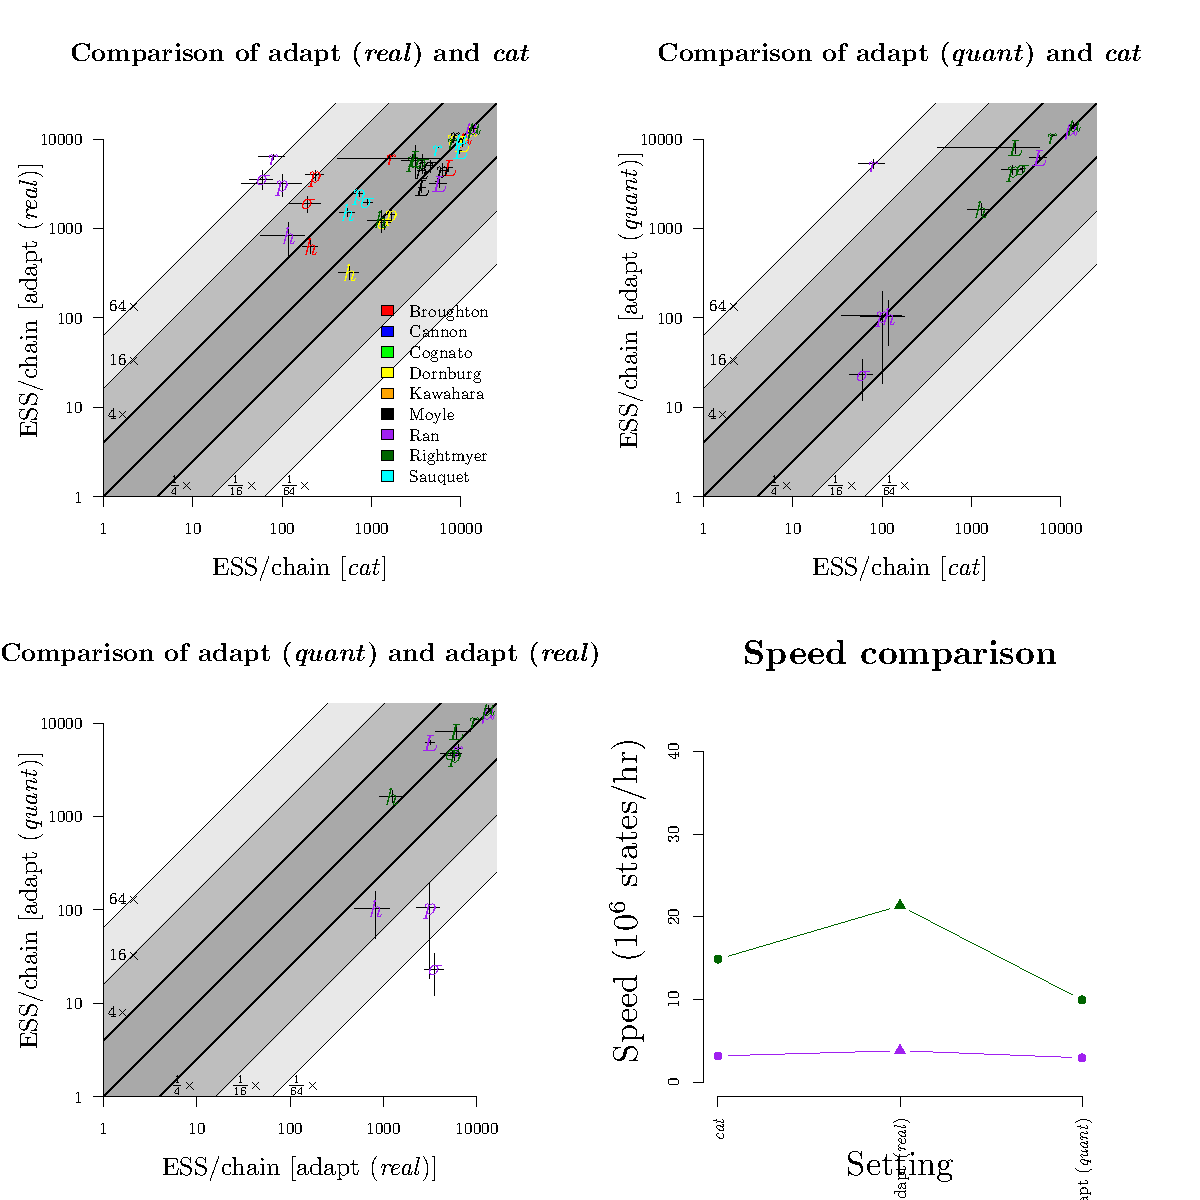
\includegraphics[width=\textwidth]{/home/jdou557/Documents/Marsden2019/Months/July2020/fromVM/benchmarkingVM/ESS_round1.pdf}
\caption{\textbf{Rate parameterisation performance evaluation.} Comparison of ESS/hr (averaged across five independent MC3 analyses) with respect to relevant terms -- $P$: posterior density; $L$: likelihood, $p$: prior density, $r$: clock rate ESS averaged across all leaves, $\hat{r}$: branch rate mean, $v$: branch rate variance, $\sigma$: clock standard deviation, $\kappa$: HKY model transition-transversion ratio, $\lambda$: Yule model birth rate. $h$: tree height. Datasets are displayed in \textbf{Table \ref{table:datasets}}.  }
\label{fig:parameterisationResults}
\end{figure}




% 1-3) the \textit{cat}, \textit{real}, and \textit{quant} parameterisations using the operators described by Drummond et al. 2006 \cite{drummond2006relaxed}; 3) the \textit{quant} parameteristion 



\subsection*{Round 3: Bactrian proposal kernels are 10\% more efficient than uniform kernels}



\subsection*{Round 4: Finding the best NER operator variant}

The \textbf{\nameref{sect:NER}} (NER) operators are evaluated. This protocol selects the best among 48 NER (no random walk) and 48 NERw ($\text{Bactrian}(0.95)$ random walk) operators, and has two phases. First, the best of the 96 is selected by comparing operator acceptance rates on simulated data. Second, the selected operator is benchmarked with respect to convergence time and sampling rate on real data (\textbf{Table \ref{table:datasets}}). The analyses in this section invoke the \textit{quant} parameterisation and $\text{Bactrian}(0.95)$ proposal kernels on clock model parameters.




\subsubsection*{Initial screening by acceptance rate on simulated data}


We selected the best operator variant by performing MCMC on 300 simulated datasets, where each MCMC employed all 96 NER/NERw variants. Simulated datasets have $N=30$ taxa and an alignment with $L \sim \text{Uniform}(10^2, 10^4)$ sites. The acceptance rate of each operator is compared to that of the null operator $\text{NER}\{\}$ (i.e. \texttt{Narrow Exchange}). 


\textbf{Fig. \ref{fig:acceptanceRateScreening}} shows that NER variants which satisfy the genetic distances between nodes $B$ and $A$ (i.e. $\mathcal{D}_{AB}$) or between $B$ and $C$ (i.e. $\mathcal{D}_{BC}$) usually perform worse than the standard \texttt{Narrow Exchange} operator, where $B$ is the node being interchanged from the $A$ branch to the $C$ branch (\textbf{Fig. \ref{fig:narrowexchange}}). 
This is an intuitive result. 
If the posterior distribution is relatively flat, and the data presents high uncertainty in the positioning of $B$, with respect to $A$ and $C$, then the topological rearrangement performed by \texttt{Narrow Exchange} will be favoured. However, this uncertainty in the \textit{topology} is likely coupled with uncertainty in the \textit{distance} between $B$ and $A$ or between $B$ and $C$. 
Thus, in this case, respecting the $\mathcal{D}_{AB}$ and $\mathcal{D}_{BC}$ constraints (by proposing branch rates) makes too many unnecessary changes to the state and the operator performs worse.



\begin{figure}[!h]
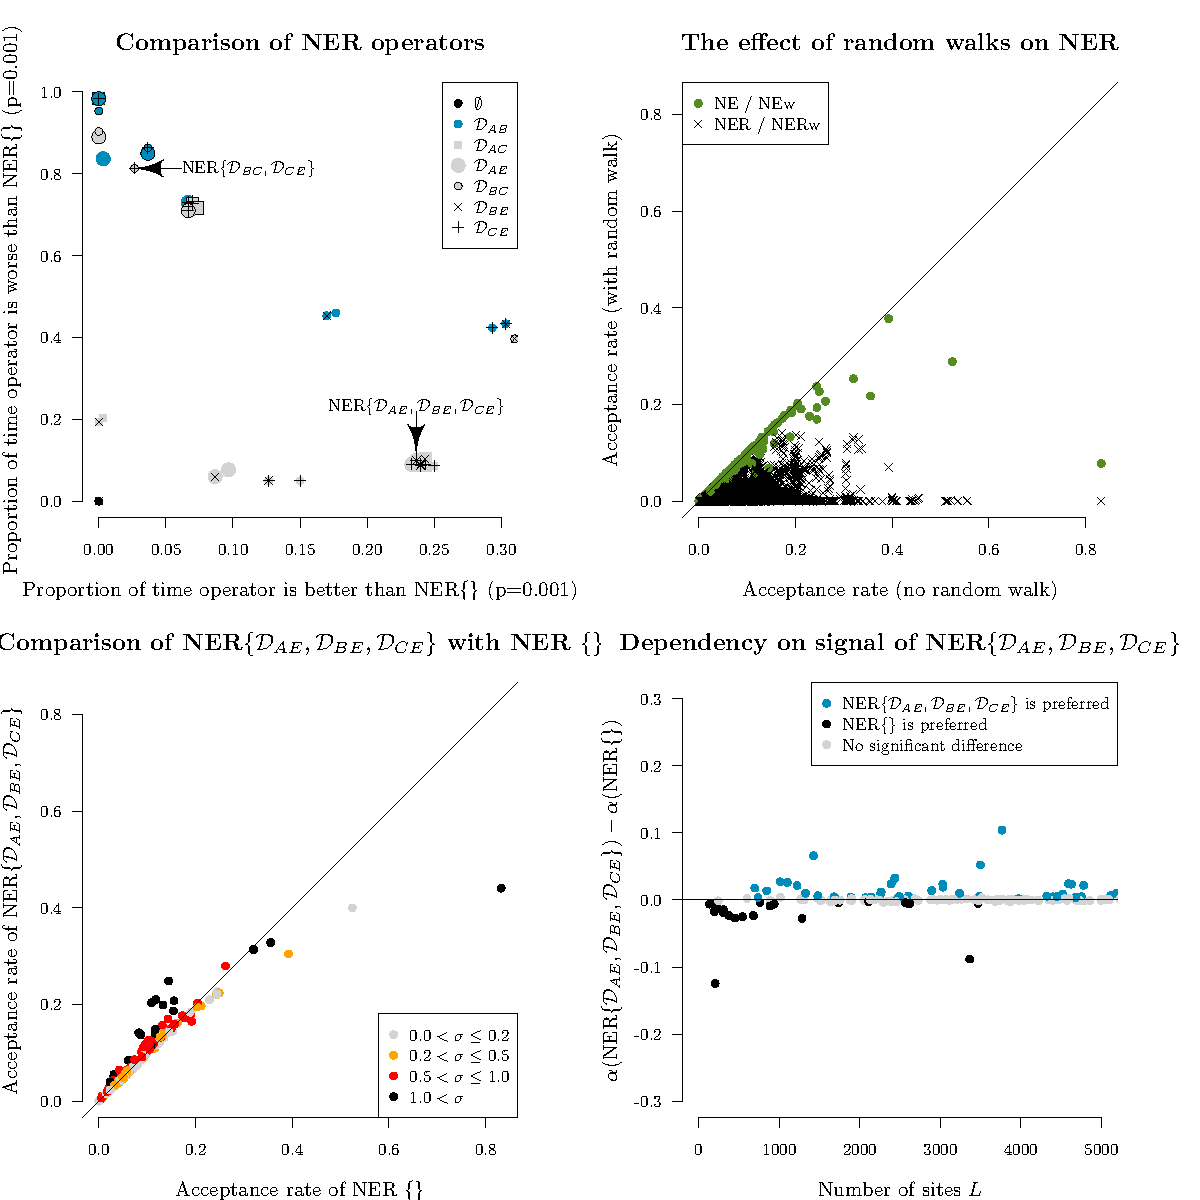
\includegraphics[width=\textwidth]{Figures/acceptanceRates.pdf}
\caption{\textbf{Screening of NER and NERw variants by acceptance rate.} Top left: comparison of NER variants with the null operator $\text{NER}\{\}$ (i.e. \texttt{NarrowExchange}). Each of the 48 operators are represented by a single point, uniquely encoded by the point stylings. The number of times each operator is proposed and accepted is compared with that of $\text{NER}\{\}$, and one-sided z-tests are performed to assess the statistical significance between the two acceptance rates ($p = 0.001$).  This process is repeated for each of $300$ simulated datasets. The axes of each plot are the proportion of these $300$ simulations for which there is evidence that the operator is significantly better than $\text{NER}\{\}$ (x-axis) or worse than $\text{NER}\{\}$ (y-axis). Top right: comparison of NER and NERw acceptance rates. Each point is one NER/NERw variant from a single simulation. Bottom: relationship between the acceptance rates $\alpha$ of $\text{NER}\{\mathcal{D}_{AE}, \mathcal{D}_{BE}, \mathcal{D}_{CE}\}$ and $\text{NER}\{ \}$ with the clock model standard deviation $\sigma$ and the number of sites $L$.  Each point is a single simulation. }
\label{fig:acceptanceRateScreening}
\end{figure}





\textbf{Fig. \ref{fig:acceptanceRateScreening}} also reveals a cluster of NER variants which -- under the conditions of the simulation --  performed better than the null operator $\text{NER}\{\}$ around 25\% of the time and performed worse around 10\% of the time. 
One such operator is  $\text{NER}\{\mathcal{D}_{AE}, \mathcal{D}_{BE}, \mathcal{D}_{CE}\}$ and is presented in \textbf{Algorithm \ref{alg:NER2}}. 
This variant conserves the genetic distance between the child nodes ($A, B, C$) and the grandparent node $E$. This is performed by proposing rates for $r_A$, $r_B$, and $r_C$ while obeying the distance constraints imposed by the operator. Exploring this operator further, we can see that $\text{NER}\{\mathcal{D}_{AE}, \mathcal{D}_{BE}, \mathcal{D}_{CE}\}$ is at its best when there is a large variance in branch rate i.e. when clock standard deviation $\sigma$ is high ($\sigma \gtrsim 0.5$ for $N=30$), corresponding to data which is not clock-like. On the other hand, $\text{NER}\{\}$ is much preferred when the operator's acceptance rate is high ($\gtrsim 0.15$) -- corresponding to datasets with short sequences ($L < 1$kb for $N=30$) and thus poor signal.  
Overall, $\text{NER}\{\mathcal{D}_{AE}, \mathcal{D}_{BE}, \mathcal{D}_{CE}\}$ outperforms the standard \texttt{NarrowExchange} operator when the data is not clock-like and contains enough signal. 




Finally, \textbf{Fig. \ref{fig:acceptanceRateScreening}} shows that by applying a (Bactrian) random walk to $t_D$ -- the height of internal node $D$ -- the acceptance rate of NER plummets dramatically. 
This effect is most dominant for the NER variants which satisfy distance constraints (i.e. the operators which are not $\text{NER}\{\}$). This result is unfortunate however not unexpected, and is consistent with Lakner et al. 2008 \cite{lakner2008efficiency}, who observed that tree operators perform best when they change either topology, or branch lengths, but not both.



Although there are several operators which are tying for first place and behave equivalently, we selected the $\text{NER}\{\mathcal{D}_{AE}, \mathcal{D}_{BE}, \mathcal{D}_{CE}\}$ operator to proceed to the next round of optimisation.





\subsubsection*{Benchmarking convergence time}




\subsection*{Round 5: The AVMVN leaf rate operator works well for small taxon sets}





\section*{Discussion} \label{sect:discussion}






\begin{figure}[!h]
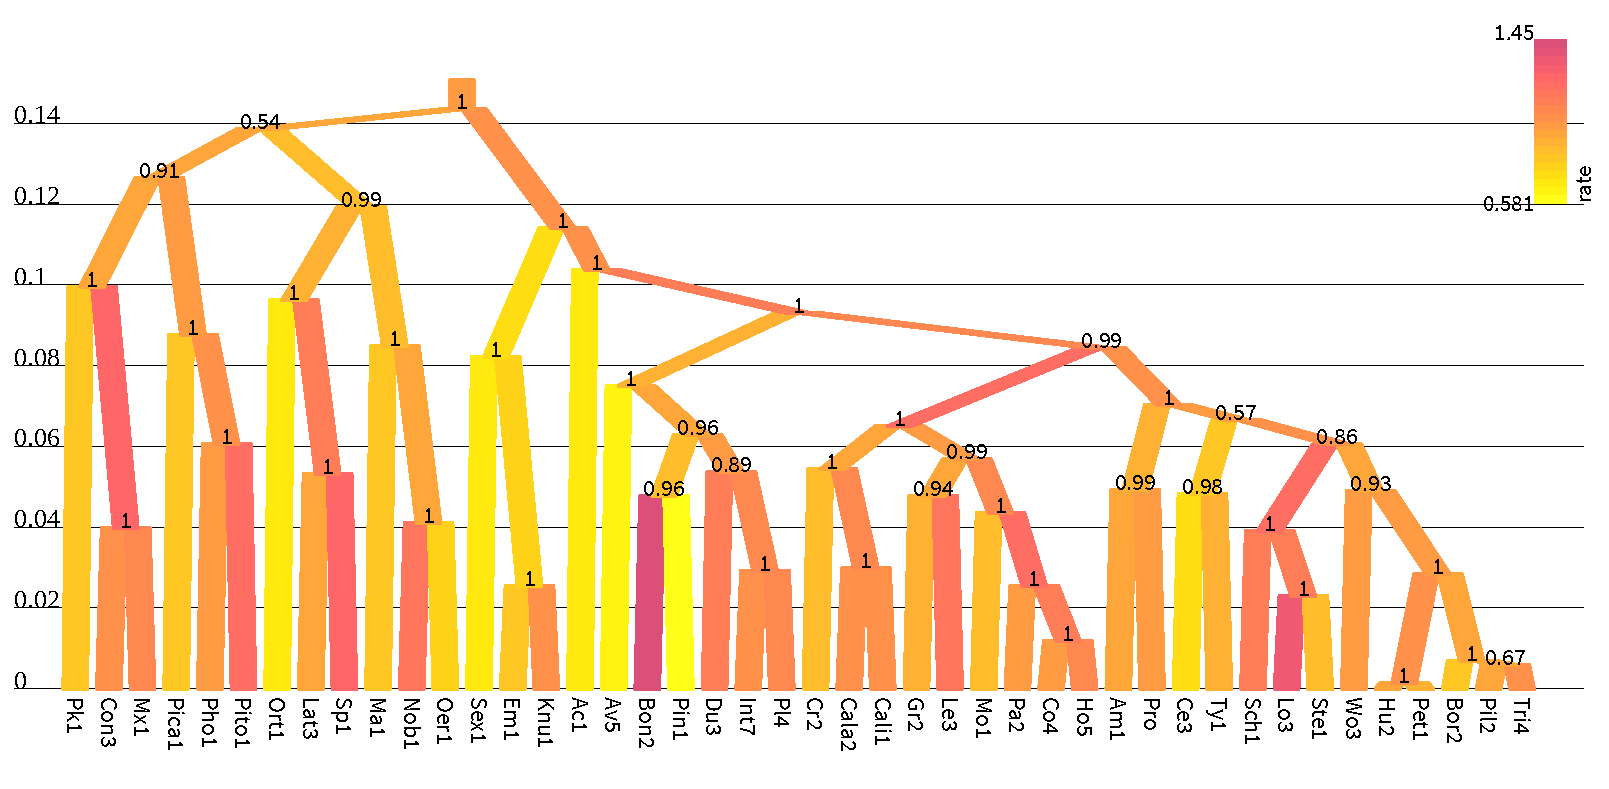
\includegraphics[width=\textwidth]{Figures/cognato.pdf}
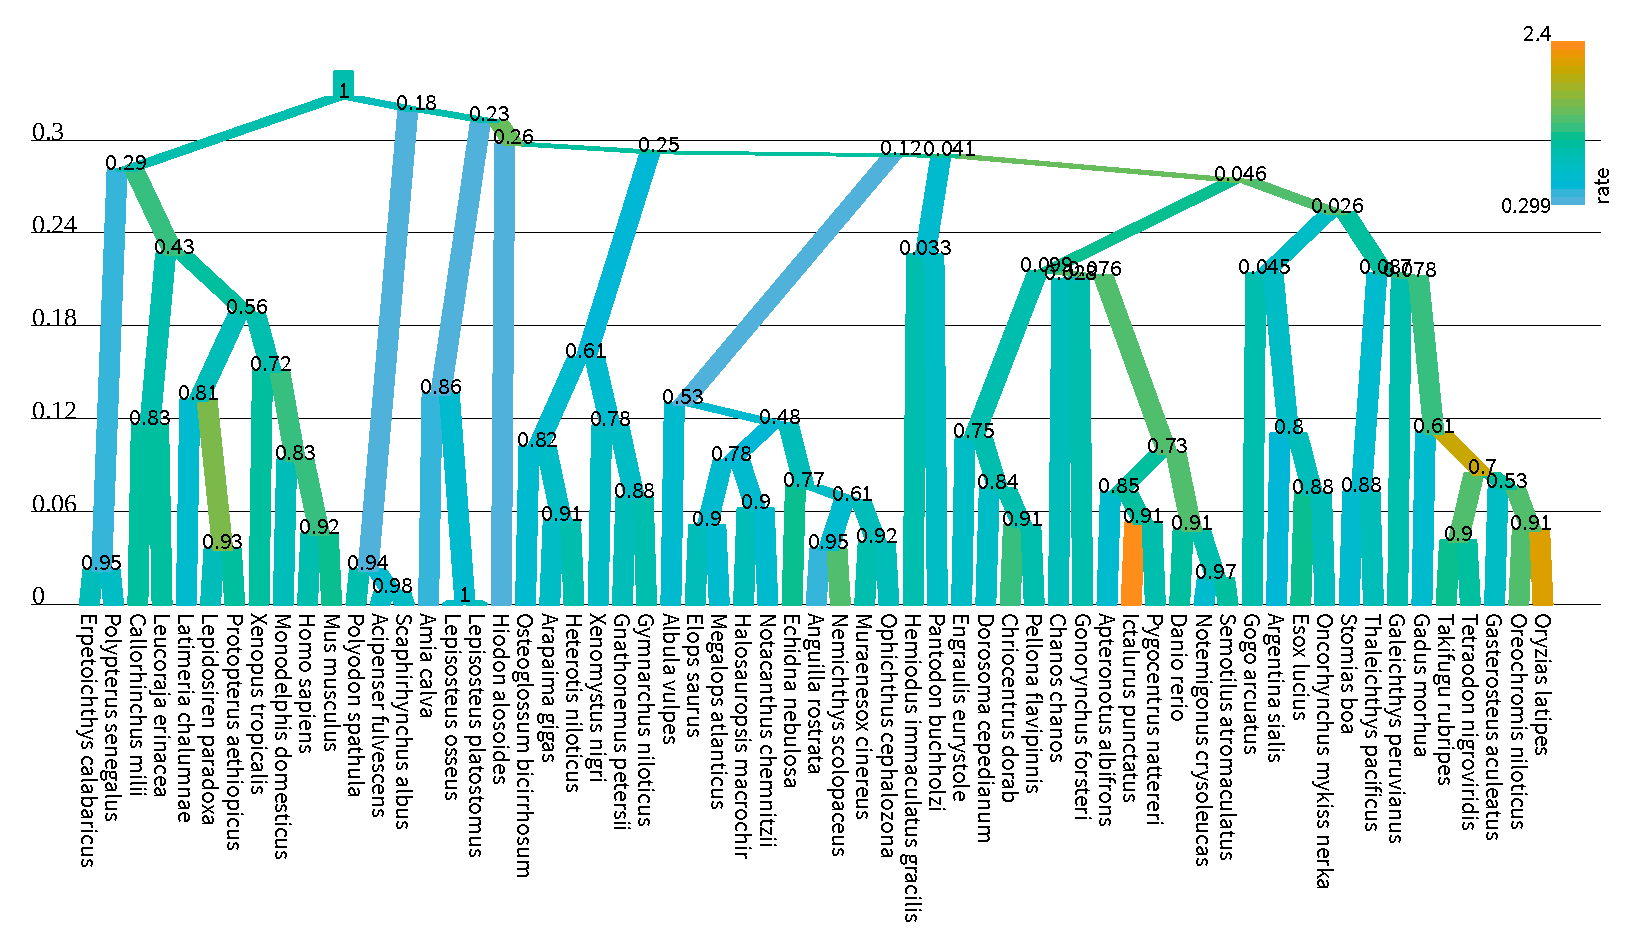
\includegraphics[width=\textwidth]{Figures/broughton.pdf}
\caption{\textbf{Maximum clade credibility trees.} Trees from the bark beetle data by Cognato et al. 2001 \cite{Cognato_2001} (top) and the bony fish data by Broughton et al. 2013 \cite{Broughton_2013} (bottom) are presented above. Branches are coloured by substitution rate (units: substitutions per site per unit of time) and the y-axis shows arbitrary units of time. Internal nodes are labelled with posterior clade support. Figures generated by UglyTrees \cite{uglytrees}.  }
\label{fig:parameterisationResults}
\end{figure}






\section*{Conclusion}


\newpage
\section*{Supporting information}


\paragraph*{S1 Appendix.}
\label{sect:S1Appendix}
{\textbf{Rate quantiles.} The linear piecewise approximation used in the \textit{quant} parameterisation is described. \texttt{Constant distance} tree operators \cite{zhang2020improving} are extended to the \textit{quant} parameterisation. 



\paragraph*{S2 Appendix.}
\label{sect:WCSS_appendix}
{\textbf{Well-calibated simulation studies.} Methodologies are validated using well-calibated simulation studies.




\nolinenumbers

% Either type in your references using
% \begin{thebibliography}{}
% \bibitem{}
% Text
% \end{thebibliography}
%
% or
%
% Compile your BiBTeX database using our plos2015.bst
% style file and paste the contents of your .bbl file
% here. See http://journals.plos.org/plosone/s/latex for
% step-by-step instructions.
%

\newpage
\bibliography{references}



\end{document}












